\documentclass[]{article}
\usepackage{lmodern}
\usepackage{amssymb,amsmath}
\usepackage{ifxetex,ifluatex}
\usepackage{fixltx2e} % provides \textsubscript
\ifnum 0\ifxetex 1\fi\ifluatex 1\fi=0 % if pdftex
  \usepackage[T1]{fontenc}
  \usepackage[utf8]{inputenc}
\else % if luatex or xelatex
  \ifxetex
    \usepackage{mathspec}
  \else
    \usepackage{fontspec}
  \fi
  \defaultfontfeatures{Ligatures=TeX,Scale=MatchLowercase}
\fi
% use upquote if available, for straight quotes in verbatim environments
\IfFileExists{upquote.sty}{\usepackage{upquote}}{}
% use microtype if available
\IfFileExists{microtype.sty}{%
\usepackage{microtype}
\UseMicrotypeSet[protrusion]{basicmath} % disable protrusion for tt fonts
}{}
\usepackage[margin=1in]{geometry}
\usepackage{hyperref}
\hypersetup{unicode=true,
            pdfborder={0 0 0},
            breaklinks=true}
\urlstyle{same}  % don't use monospace font for urls
\usepackage{graphicx,grffile}
\makeatletter
\def\maxwidth{\ifdim\Gin@nat@width>\linewidth\linewidth\else\Gin@nat@width\fi}
\def\maxheight{\ifdim\Gin@nat@height>\textheight\textheight\else\Gin@nat@height\fi}
\makeatother
% Scale images if necessary, so that they will not overflow the page
% margins by default, and it is still possible to overwrite the defaults
% using explicit options in \includegraphics[width, height, ...]{}
\setkeys{Gin}{width=\maxwidth,height=\maxheight,keepaspectratio}
\IfFileExists{parskip.sty}{%
\usepackage{parskip}
}{% else
\setlength{\parindent}{0pt}
\setlength{\parskip}{6pt plus 2pt minus 1pt}
}
\setlength{\emergencystretch}{3em}  % prevent overfull lines
\providecommand{\tightlist}{%
  \setlength{\itemsep}{0pt}\setlength{\parskip}{0pt}}
\setcounter{secnumdepth}{0}
% Redefines (sub)paragraphs to behave more like sections
\ifx\paragraph\undefined\else
\let\oldparagraph\paragraph
\renewcommand{\paragraph}[1]{\oldparagraph{#1}\mbox{}}
\fi
\ifx\subparagraph\undefined\else
\let\oldsubparagraph\subparagraph
\renewcommand{\subparagraph}[1]{\oldsubparagraph{#1}\mbox{}}
\fi

%%% Use protect on footnotes to avoid problems with footnotes in titles
\let\rmarkdownfootnote\footnote%
\def\footnote{\protect\rmarkdownfootnote}

%%% Change title format to be more compact
\usepackage{titling}

% Create subtitle command for use in maketitle
\newcommand{\subtitle}[1]{
  \posttitle{
    \begin{center}\large#1\end{center}
    }
}

\setlength{\droptitle}{-2em}
  \title{}
  \pretitle{\vspace{\droptitle}}
  \posttitle{}
  \author{}
  \preauthor{}\postauthor{}
  \date{}
  \predate{}\postdate{}


\begin{document}

After discussing available data sources and measurement approaches, it
seems worthwhile to compare them empirically as well. This chapter
introduces the examined measurements, explains the many ways the data
had to be transformed in order to reproduce some of the previously
discussed measurements, and therefore may serve as an example to
researchers interested in measuring direct democracy with the given
data. Subsequently the reconstruction of the selected direct democracy
measures is described (Section \ref{data_wrangling}). Following that, we
empirically compare the indicators of rules in form (\ref{rif_empiric})
and rules in use (Section \ref{riu_empiric}) as well as measures that
include both (Section \ref{mixed_empiric}) separately.

\subsection{Data Wrangling} \label{data_wrangling}

This section elaborates on the various transformations that had to be
applied in order to reproduce the selected measurement approaches. It
further introduces the ready-to-use variables taken from other sources.
First, the rules in form measures are discussed, followed by the rules
in use indicators and the mixed approaches.

\subsubsection{Construction of Rules in Form
Measures}\label{construction-of-rules-in-form-measures}

First, we consider how the different rules in form measures were
constructed. In order to make the measures comparable, we use the most
recent data available for each dataset. In total, there are three rules
in form measures to be constructed: Gherghina - Rif, \emph{Peters - RiF}
and \emph{V-Dem RiF}, with respective bottom-up and top-down components
when available. Additionally, two indicators will also be used in order
to enhance the comparison: \emph{Direct Democracy Provisions} from the
Democracy Barometer and \emph{Direct Democracy Legal Designs} from the
Direct Democracy Navigator. Table \ref{rif_table} shows descriptives
statistics for the used measures.

\begin{table}[!h]
\centering
\caption{Rules in Form}
\label{rif_table}
\resizebox{\textwidth}{!}
{\begin{tabular}{lccccccc}
  \toprule
\textbf{Rules in Form Measures} & \textbf{N(=Countries)} & \textbf{Mean} & \textbf{SD} & \textbf{Median} & \textbf{Range} & \textbf{Time} & \textbf{Data} \\ 
  \midrule
Gherghina - RiF & 192 & 1.76 & 1.24 & 2.00 & 0 - 5 & Most Recent & IDEA \\ 
  Peters - RiF & 196 & 0.62 & 0.46 & 0.50 & 0 - 1.5 & '' & '' \\ 
  \hskip .5cm \textit{Top-Down} & 196 & 0.80 & 0.53 & 1.00 & 0 - 1.5 & '' & '' \\ 
   \hskip .5cm \textit{Bottom-Up} & 196 & 0.44 & 0.64 & 0.00 & 0 - 1.5 & '' & '' \\ 
  V-Dem - RiF & 170 & 1.64 & 1.06 & 2.00 & 0 - 4 & 2016 & V-Dem \\ 
  \hskip .5cm \textit{Top-Down} & 172 & 1.26 & 0.69 & 1.00 & 0 - 2 & '' & '' \\ 
  \hskip .5cm \textit{Bottom-Up} & 170 & 0.38 & 0.71 & 0.00 & 0 - 2 & '' & '' \\ 
  Direct Democracy Provisions & 68 & 1.65 & 1.38 & 1.33 & 0 - 4 & 2014 & Democracy Barometer \\ 
  Direct Democracy Legal Designs & 107 & 2.86 & 1.94 & 2.00 & 1 - 12 & Most Recent & Direct Democracy Navigator \\ 
   \bottomrule
\end{tabular}}
\end{table}

\clearpage

\paragraph{Gherghina - RiF}\label{gherghina---rif}

As already discussed in the previous chapter, the Gherghina Rules in
Form (referred to as: \emph{Gherghina - RiF}) measure is a simple count
of the given direct democracy mechanisms available in the IDEA dataset:
mandatory/obligatory referendums, optional referendums, citizens
initiatives, agenda initiatives and recall. This is easily reproduced
for all available countries in the IDEA dataset. IDEA includes a column
for each mechanism \emph{''Legal provisions for {[}mechanism{]} at
national level}'', indicating whether ``Yes'' the respective provision
is available in that country on the national level and ``No'' for when
the measure is not available. In accordance with general practice, cases
with ``Yes'' are coded as 1 and cases with ``No'' are coded as 0. A
special case is when certain countries specify a condition such as ``No,
but ad hoc referendums are possible'' (for example in Norway for
optional referendums). It was decided to classify such cases as a ``No''
(= 0), as an ad hoc referendum implies that there generally is no legal
basis on which a referendum can occur and therefore it is not an
indicator of rules in form. Cases indicating ``No data'' are coded
appropriately as missing value. As a next step the five variables are
simply counted, leading to a 6-point scale ranging from 0 to 5, where 0
indicates that there are no provisions in place in that country and 5
means that all 5 of them are in place. Data was available for 192
countries and the average amount of provisions in place was 1.76 (SD =
1.24).\footnote{As this paper focuses on the national level, we refer
  from reconstructing Gherghinas' index for the local/regional level,
  but recommend researchers to use the IDEA dataset if interested in
  doing so.}

\paragraph{Peters - RiF}\label{peters---rif}

Next, it is described how the rules in form measure by @peters2016 is
constructed (referred to as: \emph{Peters - RiF}). In order to calculate
the Peters - RiF measure, IDEA is again the most appropriate dataset as
it offers information on agenda initiatives and the aim of this
reconstruction is to stay as close as possible to the original measure.
As a first step, the column \emph{''Who can initiate an optional
referendum at the national level?''} will be parsed in order to extract
information on the bottom-up or top-down nature of a optional referendum
in a given country. Whenever a case includes the phrase ``Registered
Electors'', the variable is coded as \emph{Bottom-Up} and whenever a
case includes a state institution (``Government'', ``Supreme Court'',
``Parliament'' etc.) it is coded as \emph{Top-Down}. The phrase ``Not
applicable'' is coded as 0 in either case, as it implies that there is
no obligatory referendum in that country in the first place, and again
``No data'' is coded as missing value.

Next, the bindingness of a given referendum is coded. The column
\emph{``Are referendum results binding?''} includes information on the
bindingness of referendums. Whenever the phrase ``Optional referendum -
always'' appears, the specific country receives a 1 for optional
referendum decisiveness, whereas ``Optional referendum - never'' and
``Optional referendum - sometimes'' is classified as non-binding. We
consider sometimes binding referendums as generally non-binding, as
bindingness in that case depends on other factors (such as ease of
approval).\footnote{A different approach worth considering would be to
  give sometimes binding referendums a medium score. As we want to stay
  as close as possible to the original index construction by Peters -
  RiF, we decided to use the mentioned approach.} Now the variables are
in place in order to construct the top-down following @peters2016.
Whenever a country has a \emph{binding} optional referendum that is
initiated by state institutions, it receives a score of 1, while a
country with a \emph{non-binding} top-down initiated optional referendum
receives a score of 0.5, creating the variable \emph{legislative
referendum} equivalent to the @peters2016 measure with the same name.
Similarly, whenever there is a mandatory referendum in a given country,
it receives the score of 2, otherwise a 0, creating the variable
\emph{constitutional referendum} equally constructed as the @peters2016
variable with the same name. Subsequently, the the top-down measure can
be constructed by adding up constitutional referendum and legislative
referendum divided by 2, which results in a 0 to 1.5 scale.

For the bottom-up measure, a variable ``citizens initiative'' is
calculated, which takes the value 3 if a citizens' initiative exists and
0 if not.\footnote{As a departure from @peters2016, we refrain from
  assigning a 1.5 category, as parsing and coding individual issues for
  each citizen or agenda initiative is a task that would require
  researching each initiative individually, something that is beyond the
  scope of this paper.} The variable ``agenda initiative'' takes the
value 1 if an agenda initiative is provided and 0 if not. The aggregated
bottom up measure is constructed by adding both variables and dividing
by 3, also resulting in a 0 to 1.5 scale. It has to be noted, that we
are not sure whether this construction corresponds to the calculation as
intended by Peters (see Chapter \ref{measurement} for the discussion of
the other possible construction method).

As a final step, Peters - RiF is constructed by adding up the top-down
and the bottom-up measures and dividing them by two, creating yet
another 0 to 1.5 scale. The average Peters - RiF score is 0.62 (SD =
0.46). The average top-down score of the Peters - RiF measure is 0.80
(SD = 0.53), whereas the average Bottom-Up score is 0.44 (SD = 0.64),
already implying that there are more top-down rules in form on average .
The three measures are available for 196 countries.

\paragraph{V-Dem RiF}\label{v-dem-rif}

The V-Dem rules in form measures (referred to as: \emph{V-Dem RiF}) are
an attempt to emulate the approach taken in @gherghina2016, meaning,
it's a simple count index of the four direct democracy mechanisms that
are available in the V-Dem dataset: obligatory referendums, plebiscites,
initiatives and (facultative) referendums. This leads to a four-point
scale, where 0 means no democracy mechanism is in place, whereas 4 means
that all four legal provisions are in place. An advantage of the V-Dem
data is that we can clearly distinguish between top-down and bottom-up
mechanism. Therefore, we calculated a V-Dem - RiF top-down measure by
summing obligatory referendums and plebiscites provisions (3-point
measure) and a bottom-up measure by summing initiatives and facultative
referendums (also a 3-point measure). On average there were 1.64
provisions in place (SD = 1.06), while the higher average value for
top-down (Mean = 1.26, SD = 0.69) compared to bottom-up (Mean = 0.38, SD
= 0.71) implies a greater prevalence of top-down rules in form measures.
The V-Dem RiF measure and its bottom-up component are available for 170
countries, whereas the top-down component is available for 172
countries.

\paragraph{Democracy Barometer and Direct Democracy Navigator
Indicators}\label{democracy-barometer-and-direct-democracy-navigator-indicators}

The following indicators are taken from their respective data sources:
\emph{Direct Democracy Provisions} from the Democracy Barometer and
\emph{Direct Democracy Legal Designs} from the Direct Democracy
Navigator. Direct Democracy Provisions are available for 68 countries
and similarly to @gherghina2016 it is a simple count measure of direct
democratic provisions, with an average of 1.65 (SD = 1.38) measures in
place. Direct Democracy Legal Designs is a simple count of legal designs
for direct democratic institutions available in a given country. As
already discussed in Chapter \ref{data}, some inconsistencies can be
observed when delving deeper into the database. However, we still
consider it to be a valuable data source that is at least worthy of
comparison. The average use of legal designs is 2.86 (SD = 1.94) and the
measure is available for 107 countries. Note that the Direct Democracy
Navigator does not distinguish between a country not having any
provisions at all or a completely missing case, therefore there is no 0
category and only countries are recorded that have at least one legal
design on the national level.

\subsubsection{Construction of Rules in Use
Measures}\label{construction-of-rules-in-use-measures}

Next, we will discuss how the rules in use measures were created. In
order to facilitate comparison, we limit the data to a common (rather
large) time range, as referendums are not very frequent in some
countries, but still practiced occasionally. All rules in use measures
were thus aggregated for a time-frame of 21 years (1996 - 2016), except
for the Democracy Barometer data which was only available from 1996 to
2014. Table \ref{riu_table} shows descriptives statistics for the
constructed indicators.

\begin{table}[ht]
\centering
\caption{Rules in Use}
\label{riu_table}
\resizebox{\textwidth}{!}
{\begin{tabular}{lccccccc}
  \toprule
\textbf{Rules in Use Measures} & \textbf{N(=Countries)} & \textbf{Mean} & \textbf{SD} & \textbf{Median} & \textbf{Range} & \textbf{Time} & \textbf{Data} \\ 
  \midrule
Gherghina - RiU & 161 & 9.38 & 46.62 & 1.00 & 0 - 552 & 1996 - 2016 & V-Dem \\ 
  V-Dem - RiU - Sum & 172 & 3.74 & 15.43 & 1.00 & 0 - 184 & '' & '' \\ 
  \hskip .5cm \textit{Top-Down} & 172 & 2.38 & 6.80 & 1.00 & 0 - 66 & '' & '' \\ 
  \hskip .5cm \textit{Bottom-Up} & 172 & 1.37 & 11.25 & 0.00 & 0 - 144 & '' & '' \\ 
  Sudd - RiU - Sum & 96 & 8.03 & 20.76 & 2.00 & 1 - 187 & '' & sudd \\ 
  \hskip .5cm \textit{Top-Down} & 93 & 5.14 & 9.10 & 2.00 & 1 - 66 & '' & '' \\ 
  \hskip .5cm \textit{Bottom-Up} & 24 & 12.21 & 29.50 & 4.00 & 1 - 146 & '' & '' \\ 
  V-Dem - RiU - Cat. & 172 & 1.10 & 1.52 & 1.00 & 0 - 5 & '' & V-Dem \\ 
  \hskip .5cm \textit{Top-Down} & 172 & 0.94 & 1.32 & 1.00 & 0 - 5 & '' & '' \\ 
  \hskip .5cm \textit{Bottom-Up} & 172 & 0.26 & 0.92 & 0.00 & 0 - 5 & '' & '' \\ 
  Sudd - RiU - Cat. & 96 & 2.29 & 1.64 & 1.00 & 1 - 5 & '' & sudd \\ 
  \hskip .5cm \textit{Top-Down} & 93 & 1.99 & 1.46 & 1.00 & 1 - 5 & '' & '' \\ 
  \hskip .5cm \textit{Bottom-Up} & 24 & 2.54 & 1.64 & 2.00 & 1 - 5 & '' & '' \\ 
  Effective Use & 71 & 0.80 & 1.88 & 0.00 & 0 - 13 & 1996 - 2014 & Democracy Barometer \\ 
  Credible Use & 172 & 1.20 & 2.65 & 0.00 & 0 - 21 & 1996 - 2016 & V-Dem \\ 
   \bottomrule
\end{tabular}}
\end{table}

\paragraph{Gherghina - RiU}\label{gherghina---riu}

The Gherghina Rules in Use measure (referred to as: \emph{Gherghina -
RiU}) will be constructed with the help of the V-Dem dataset. As a first
step, all occurrences are counted for each available direct democracy
institution: obligatory referendums, plebiscites, initiatives and
referendums. Table \ref{vdem_vars} shows all the used variables of the
V-Dem dataset.

\begin{table}[!h]
    \centering
    \caption{V-Dem Variables used for Gherghina - RiU Indicator Construction}
    \label{vdem_vars}
%   \resizebox{\textwidth}{!}{%
        \begin{tabular}{@{}lclc@{}}
            \toprule
            \multicolumn{1}{c}{} & \multicolumn{3}{c}{V-Dem Variables} \\ \midrule
            Mechanism & \multicolumn{1}{c}{Occurences} & \multicolumn{1}{c}{Quora} & Decisiveness \\ \midrule
            Obligatory Referendum & v2ddyror & \begin{tabular}[c]{@{}l@{}}Turnout Quorum: v2ddpartor\\ Approval Quorum: v2ddappor\end{tabular} & v2ddlexor \\ \midrule
            Plebiscite & v2ddyrp & \begin{tabular}[c]{@{}l@{}}Turnout Quorum: v2ddpartpl\\ Approval Quorum: v2ddapprpl\end{tabular} & v2ddlexpl \\ \midrule
            Initiative & v2ddyrci & \begin{tabular}[c]{@{}l@{}}Turnout Quorum: v2ddpartci\\ Approval Quorum: v2ddapprci\end{tabular} & v2ddlexci \\ \midrule
            (Facultative) Referendum & v2ddyrrf & \begin{tabular}[c]{@{}l@{}}Turnout Quorum: v2ddpartrf\\ Approval Quorum: v2ddapprrf\end{tabular} & v2ddlexrf \\ \bottomrule
\\[-1em]
    \multicolumn{4}{r}{%
    \begin{minipage}{9cm}%
        \flushright
        \scriptsize Source: See V-Dem Codebook (cf. Coppedge Michael et al. 2017)
    \end{minipage}%
}
        \end{tabular}%
%   }
\end{table}

As a next step, turnout and approval quora are coded into 1, when a
quorum existed, and 0, when it did not, for each of the four mechanisms
separately. Now, the quorum variable can be calculated as @gherghina2016
suggested: when both a turnout and an initiation quorum are present, the
variable is coded as 1. When a turnout quorum was present but no
approval quorum, the variable is coded as 2. And when no turnout and no
approval quorum was present, the variable was coded as 3. This leaves us
with a case that wasn't considered by Gherghina: what if there is an
approval but no turnout quorum? It was decided that this value set will
also receive a score of 2, equivalent to the opposite setup.

Following that, the decisiveness for each mechanism is also coded into
1, when a mechanism was binding, and 0, when it wasn't, so we are able
to distinguish between consultative and binding referendums. However,
given the different data structures, the formula had to be applied to
each mechanism individually. So when a mechanism was binding, the use of
that mechanism was multiplied by the respective quorum variable
calculated above. When the mechanism wasn't binding, it was first
divided by two and then multiplied by the quorum. Finally, all four
mechanisms that have been transformed individually can now be summed up,
creating the \emph{Gherghina - RiU} measure. The average score for the
Gherghina - RiU measure is 9.38 (SD = 46.62) and is available for 161
countries.\footnote{Although the interpretation of the mean should be
  done carefully here, as serious outliers like Switzerland are included
  in the data.}

\paragraph{Summed, Categorized and other Rules in Use
Measures}\label{summed-categorized-and-other-rules-in-use-measures}

\textbf{V-Dem - RiU - Sum}

The summed V-Dem Rules in Use measure (referred to as: \emph{V-Dem - RiU
- Sum}) is constructed in a straightforward fashion. It merely consists
of summing up the occurrence of any direct democracy mechanism in the
V-Dem data in the time range from 1996 to 2016. Given that we are
dealing with V-Dem data, at this place we can use the same procedure for
the bottom-up and top-down measures. All measures are available for 172
countries and the V-Dem - RiU - Sum shows an average use of 3.74 (SD =
15.43) mechanisms, whereas Top-Down mechanisms were used 2.38 (SD =
6.80) and Bottom-Up mechanisms were used 1.37 (SD = 11.25 ) times on
average.\footnote{Again the interpretation of the mean should be done
  carefully as outliers are included.}

\textbf{Sudd - RiU - Sum}

The most extensive transformation had to be done on the sudd data. This
dataset was not available for easy download at the time of writing of
this paper. The creator of the database, Beat Müller, is currently
working on simplifying the structure and making it available in XML
format, though at the time of finishing this paper, this task wasn't
accomplished yet. In the meantime, the sudd data had to be web scraped
from the website directly, which was done using the R programming
language. Given that our main interest in this paper is the spread of
direct democracy on the national level, we first excluded all
referendums from regions that were dependent at the time (mostly
colonized entities) or were held in only part of a sovereign country.
Votes held in disputed territories or regions generally not recognized
as sovereign states such as Southeast Ossetia, Crimea or the (hoax)
micronation of Sealand are also excluded. Further, the sudd data also
includes popular votes that were used to elect Prime Ministers,
Presidents, Parliamentarians and even Kings, which for the the purposes
of this comparison is not relevant and thus excluded. Lastly, we also
excluded those referendums that were categorized as ``unofficial vote'',
as there is no such category for the other compared datasets.

In order to capture the bottom-up and top-down dimensions for the sudd
data we differentiated between referendums that were initiated ``by the
people'', which were labelled as bottom-up referendums/citizens'
initiatives, and those that were initiated by either a governmental,
institutional or bureaucratic entity, which were categorized as
plebiscite/top-down referendum\footnote{For example Uruguay has
  referendums labeled as initiative, even though they weren't initiated
  by the citizens. According to our typology, these were labelled as
  top-down mechanisms}.

Lastly, all occurrences of mechanisms in the time-frame between 1996 and
2016 were summed up. On average, there were 8.03 (SD = 20.76)
occurrences of direct democracy mechanisms in 96 countries, whereas
there were 93 countries that used 5.14 (SD = 9.10) Top-Down mechanisms
and 24 countries that used 12.21 (SD = 29.50) Bottom-Up mechanisms on
average.\footnote{Once more the interpretation of the mean should be
  done carefully as outliers are included.}

Note that the sudd data is recorded on the referendum level and there is
no ``0'' category in the measurements, meaning when a direct democracy
mechanism didn't occur, it's not recorded in the data. Therefore, all
rules in use measures that use the sudd data start with 1 rather than 0
and is therefore missing for countries in which no referendum took
place.\footnote{The sudd website states that information is available
  for almost all countries in the world, indicating that a country not
  appearing in a given year really means that no referendums have taken
  place and that the case is in fact not missing. However, there is no
  obvious way to distinguish whether a case was truly missing or
  ``correctly not recorded''. On the other hand, the approach used in
  this paper has the advantage of making it possible to depict rules in
  use only for countries where they took place at least once. Especially
  the bottom-up rules in use measures are highly skewed with a large
  amount of cases having a value of 0}. That is also the reason why
there is such a high discrepancy between sample size when
differentiating between top-down and bottom-up measures, as the latter
only occurs in 24 countries in the sudd data.

\textbf{V-Dem - RiU - Categorized/Sudd - RiU - Categorized}

The V-Dem/Sudd - RiU - Categorized measures follow the example of
@bauerfatke2014, and categorize the summed occurrences of all mechanisms
into five categories (due to the longer time-frame, we extended the
threefold classification to five categories):

\vspace{0.01cm}

\begin{tabular}{p{13.5cm}}
\small
 \textit{0 = 0 occurrences}
    
 \textit{1 = 1 or 2 occurrences}
    
 \textit{2 = 3 or 4 occurrences}
    
 \textit{3 = 5 or 6 occurrences}
    
 \textit{4 = 7 or 8 occurrences}
    
 \textit{5 = 9+ occurrences}
\end{tabular}

Both the categorized sudd and V-Dem measures are available in their
top-down and bottom-up format. The average category for the overall
measures is 1.10 (SD = 1.52) for the categorized V-Dem - RiU and 2.29
(SD = 1.64) for the categorized Sudd - RiU measure. The respective means
for the top-down measures are 0.94 (SD = 1.32) for the categorized V-Dem
- RiU and 1.99(SD = 1.46) for the categorized Sudd - RiU measures. The
respective means for the bottom-up measures are 0.26 (SD = 0.92) for the
categorized V-Dem - RiU and 2.54 (SD = 1.64) for the categorized Sudd -
RiU measures. Given that only transformations were applied, data
availability for these measures is the same as in the two sections above
that use V-Dem and sudd data.

\textbf{Other Indicators}

As a means of comparison \emph{Effective Use} and \emph{Credible Use}
have been taken from their respective data sources (Democracy Barometer
and V-Dem). The effective use measure sums up the use of non-mandatory
referendums in a given year and ultimately logarithmizes the measure
``to account for the fact that an additional referendum is less
important in countries with many referenda than in countries with few
referenda'' {[}@dembarcodebook pp. 47{]}. The average effective use is
0.80 (SD = 1.88) and the measure is available for 71 countries. Finally,
the credible use measure is meant to capture the occurrence of a direct
democratic vote that is \emph{credible}, meaning that ``the official
results of the vote(s) reflect the actual vote (leaving aside issues of
voter exclusion, intimidation, or vote-buying)'' {[}@coppedge2017v pp.
151{]}. As the variable can only take the value 0 or 1 for a given year,
the maximum value for a country is 21, indicating that every year
between 1996-2016 at least one credible direct democracy mechanism
occurred. The average credible use is 1.20 (SD = 2.65) and the variable
is available for 172 countries.

\subsubsection{Mixed Measures and Additional
Variables}\label{mixed-measures-and-additional-variables}

The \emph{Direct Popular Vote Index (DPVI}) and the \emph{Direct
Democracy Index (DDI)} are taken from their respective data sources
(V-Dem and Fiorino et al. 2017). Given that @fiorino2017 created their
DDI measurement for countries in the range between 2000 and 2005, the
DPVI variable has also been averaged for this timeframe, in order to
ensure comparability. Further, the DPVI measure is also available for
its top-down (Mean = 0.20, SD = 0.20) and bottom-up components (Mean =
0.04, SD = 0.12). The overall mean DPVI score is 0.10 (SD = 0.12),
whereas the mean DDI score is 3.03 (SD = 1.83). Table \ref{mixed_table}
shows descriptives statistics for the used measures.

\begin{table}[ht]
\centering
\caption{Mixed Indices}
\label{mixed_table}
\resizebox{\textwidth}{!}
{\begin{tabular}{lccccccc}
  \toprule
\textbf{Mixed Measures} & \textbf{N(=Countries)} & \textbf{Mean} & \textbf{SD} & \textbf{Median} & \textbf{Range} & \textbf{Time} & \textbf{Data} \\ 
  \midrule
Direct Popular Vote Index (DPVI) & 172 & 0.10 & 0.12 & 0.06 & 0 - 1 & 2000 - 2005 & V-Dem \\ 
  \hskip .5cm \textit{Top-Down} & 172 & 0.20 & 0.20 & 0.11 & 0 - 1 & 2000 - 2005 & '' \\ 
  \hskip .5cm \textit{Bottom-Up} & 172 & 0.04 & 0.12 & 0.00 & 0 - 1 & 2000 - 2005 & '' \\ 
  Direct Democracy Index & 87 & 3.03 & 1.83 & 3.00 & 1 - 7 & 2000 - 2005 & Fiorino et al. 2017 \\ 
   \bottomrule
\end{tabular}}
\end{table}

\textbf{Additional variable: Freedom House Index}

As stated in the previous chapter, some autocratic or semi-democratic
regimes have adopted direct popular vote instruments, a group of
countries Altman labels the ``nightmare team'' {[}@altman2011 pp. 92{]}.
As a first exploratory application of the measures presented in this
paper, we seek to examine the rules in form, rules in use and mixed
measurement approaches for direct democracy for different regime types.
In order to do that, we use the Freedom House index {[}@fh2018freedom{]}
and its three-category classification of ``Free'', ``Partly Free'' and
``Not Free''. We then seek to descriptively evaluate whether certain
mechanism types occur in different regime types. For the rules in form
and rules in use measure, the Freedom House index is taken for the year
2016 while the mixed measures are compared to the Freedom House index of
the year 2005.

The following section compares the variables with each other: first
rules rules in form are compared, followed by a comparison of rules in
use and mixed measurements, while also accounting for top-down and
bottom-up dimensions whenever possible. In order to allow for an
intuitive visual comparison, all variables are normalized to range from
0-1. A heatmap, show the correlation between all direct democracy
assessments can be found in Appendix \ref{heatmap}.

\subsection{Comparing Rules in Form Measures} \label{rif_empiric}

In order to compare the indicators for rules in form, the bivariate
correlations are examined at first. To keep the comparison between the
measures simple, we do not visualize the relationship between all
indicators and only compare the Peters and Gherghina rules in form
measures to the other indices by depicting the regression lines, with
the drawback of some loss of information. Considering the correlations
depicted in Figure \ref{gherg_rif} and Figure \ref{peters_rif}, it can
be observed that Peters - RiF corresponds the most to Gherghina - RiF
and vice versa (r = 0.92).

\begin{figure}[!th]
    \caption{Gherghina RiF compared to other Rules in Form Measures}
    \label{gherg_rif}
    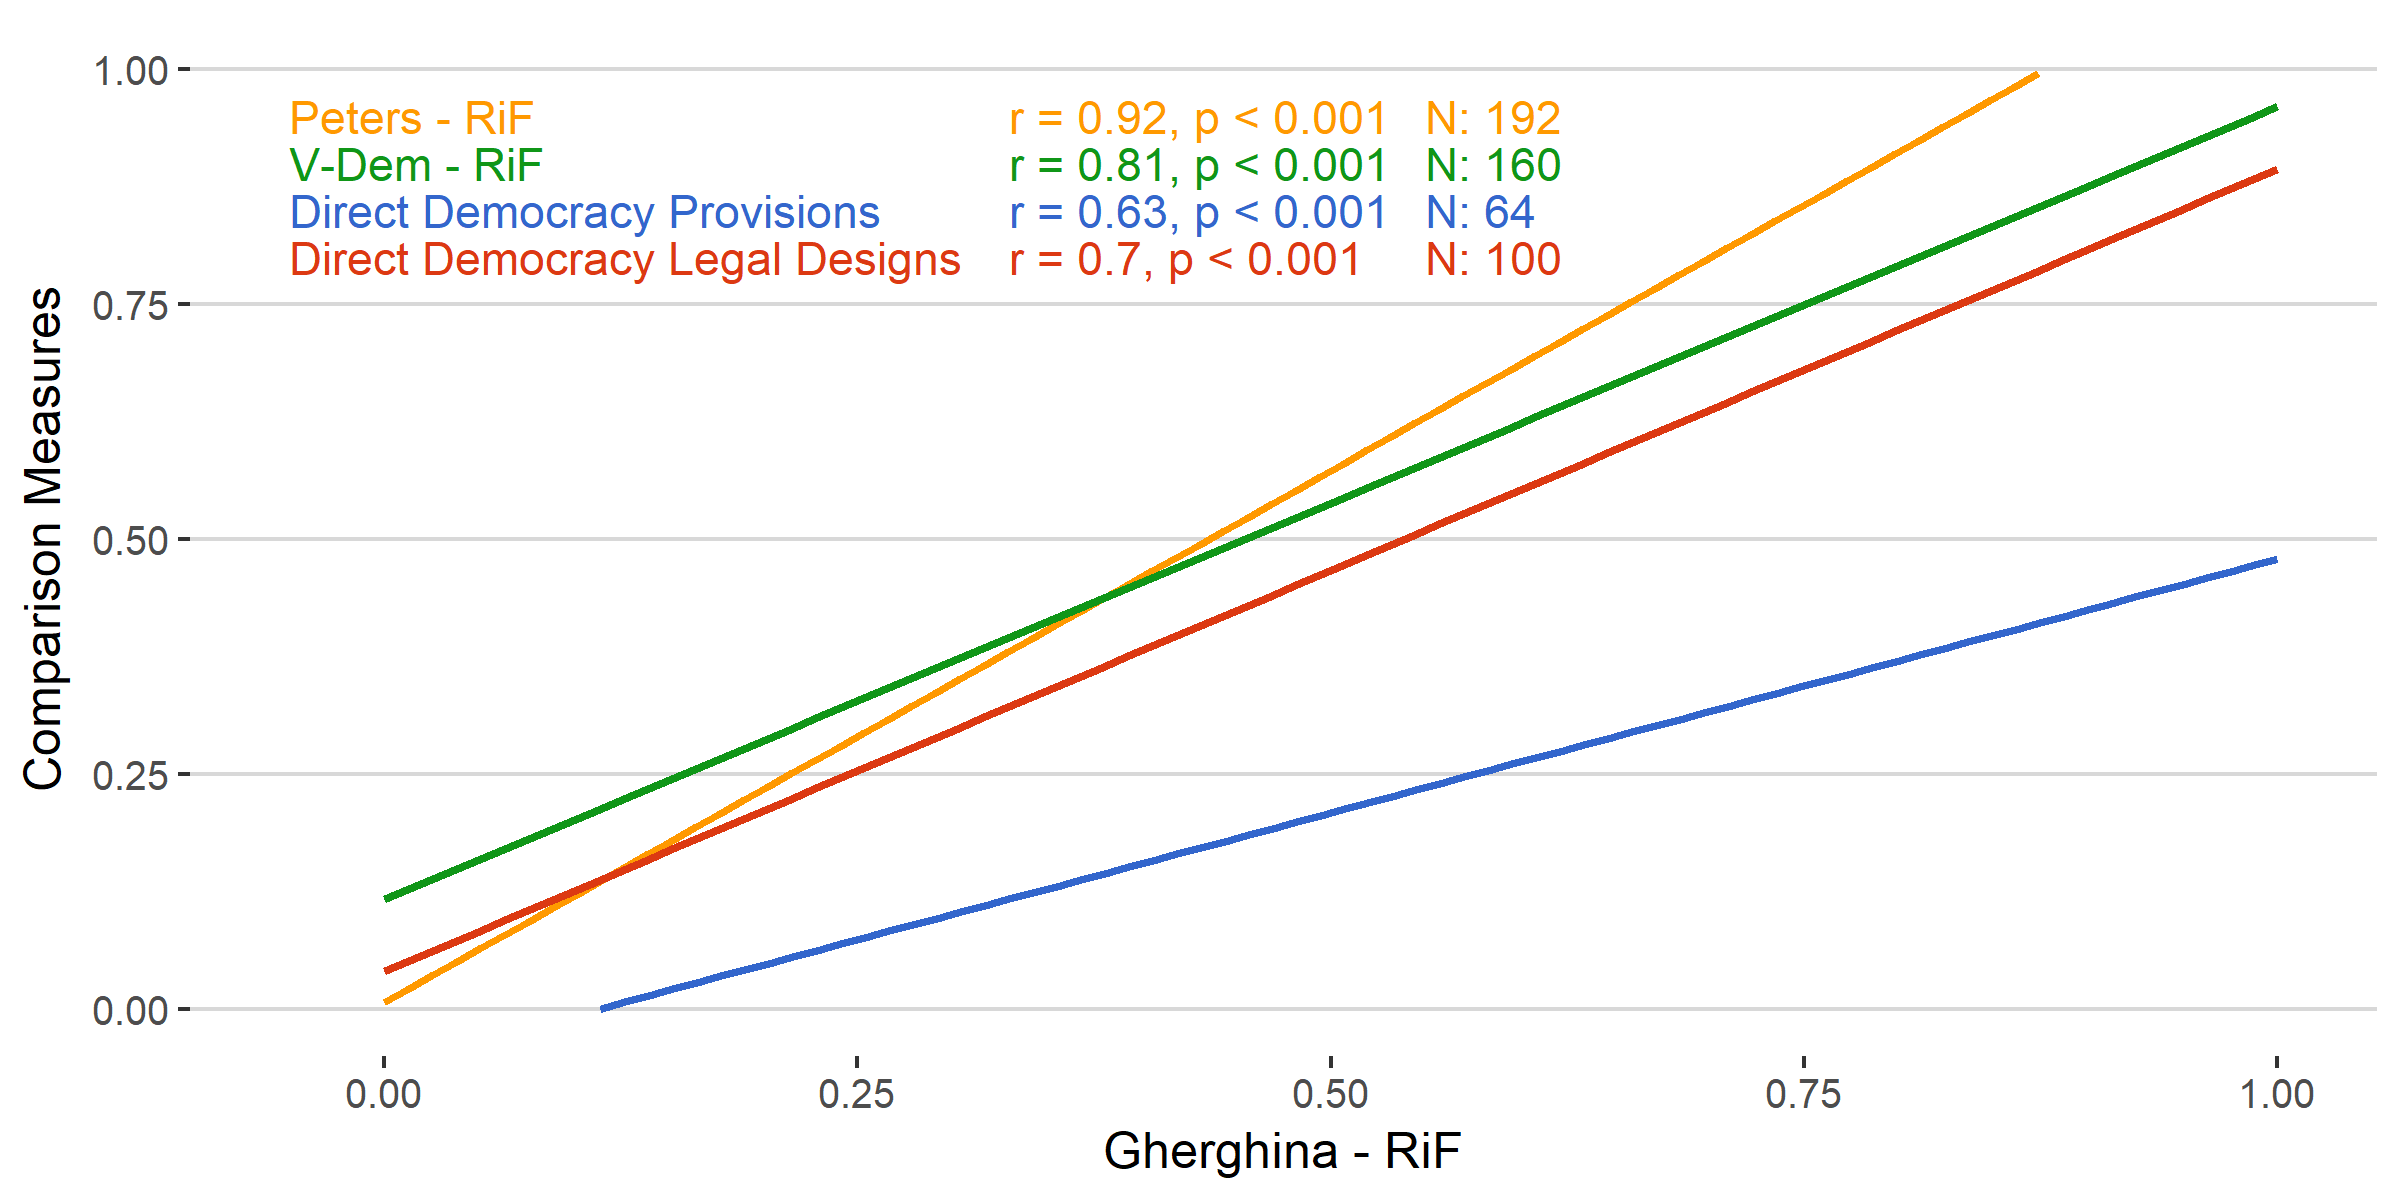
\includegraphics[width=\textwidth]{images/rif_ghergina.png}
    \flushright
    {\scriptsize Data sources: IDEA (2018), M. Coppedge et al. (2017), Navigator (2018b), Barometer (2016).\par}
\end{figure}

This is not very surprising, as they are both reconstructed using IDEA
data, even though Gherghina also considers the recall institution, while
the Peters measures gives different weights to each institution and
accounts for bindingness. The count measure constructed on the basis of
the V-Dem mechanisms (V-Dem RiF) is also closely associated with the
Gherghina index (r = 0.81), as well as the Peters measure (r = 0.78).
The Direct Democracy Provisions measure by the Democracy Barometer is
also rather strongly related to both measures, although smaller values
can be observed on the respective regression line (r \textgreater{}
0.6). This could be explained by the differing underlying typology, the
different data collection, the fact that ease of approval is accounted
for as well as the consideration of only binding mechanisms. Rather
strong correlations can also be observed with the Direct Democracy Legal
Designs variable, which is rather surprising given the fact that the
data is partly incomplete and the completely different underlying
definition of mechanisms (r \textgreater{} 0.5).

\begin{figure}[!th]
    \caption{Peters RiF compared to other Rules in Form Measures}
    \label{peters_rif}
    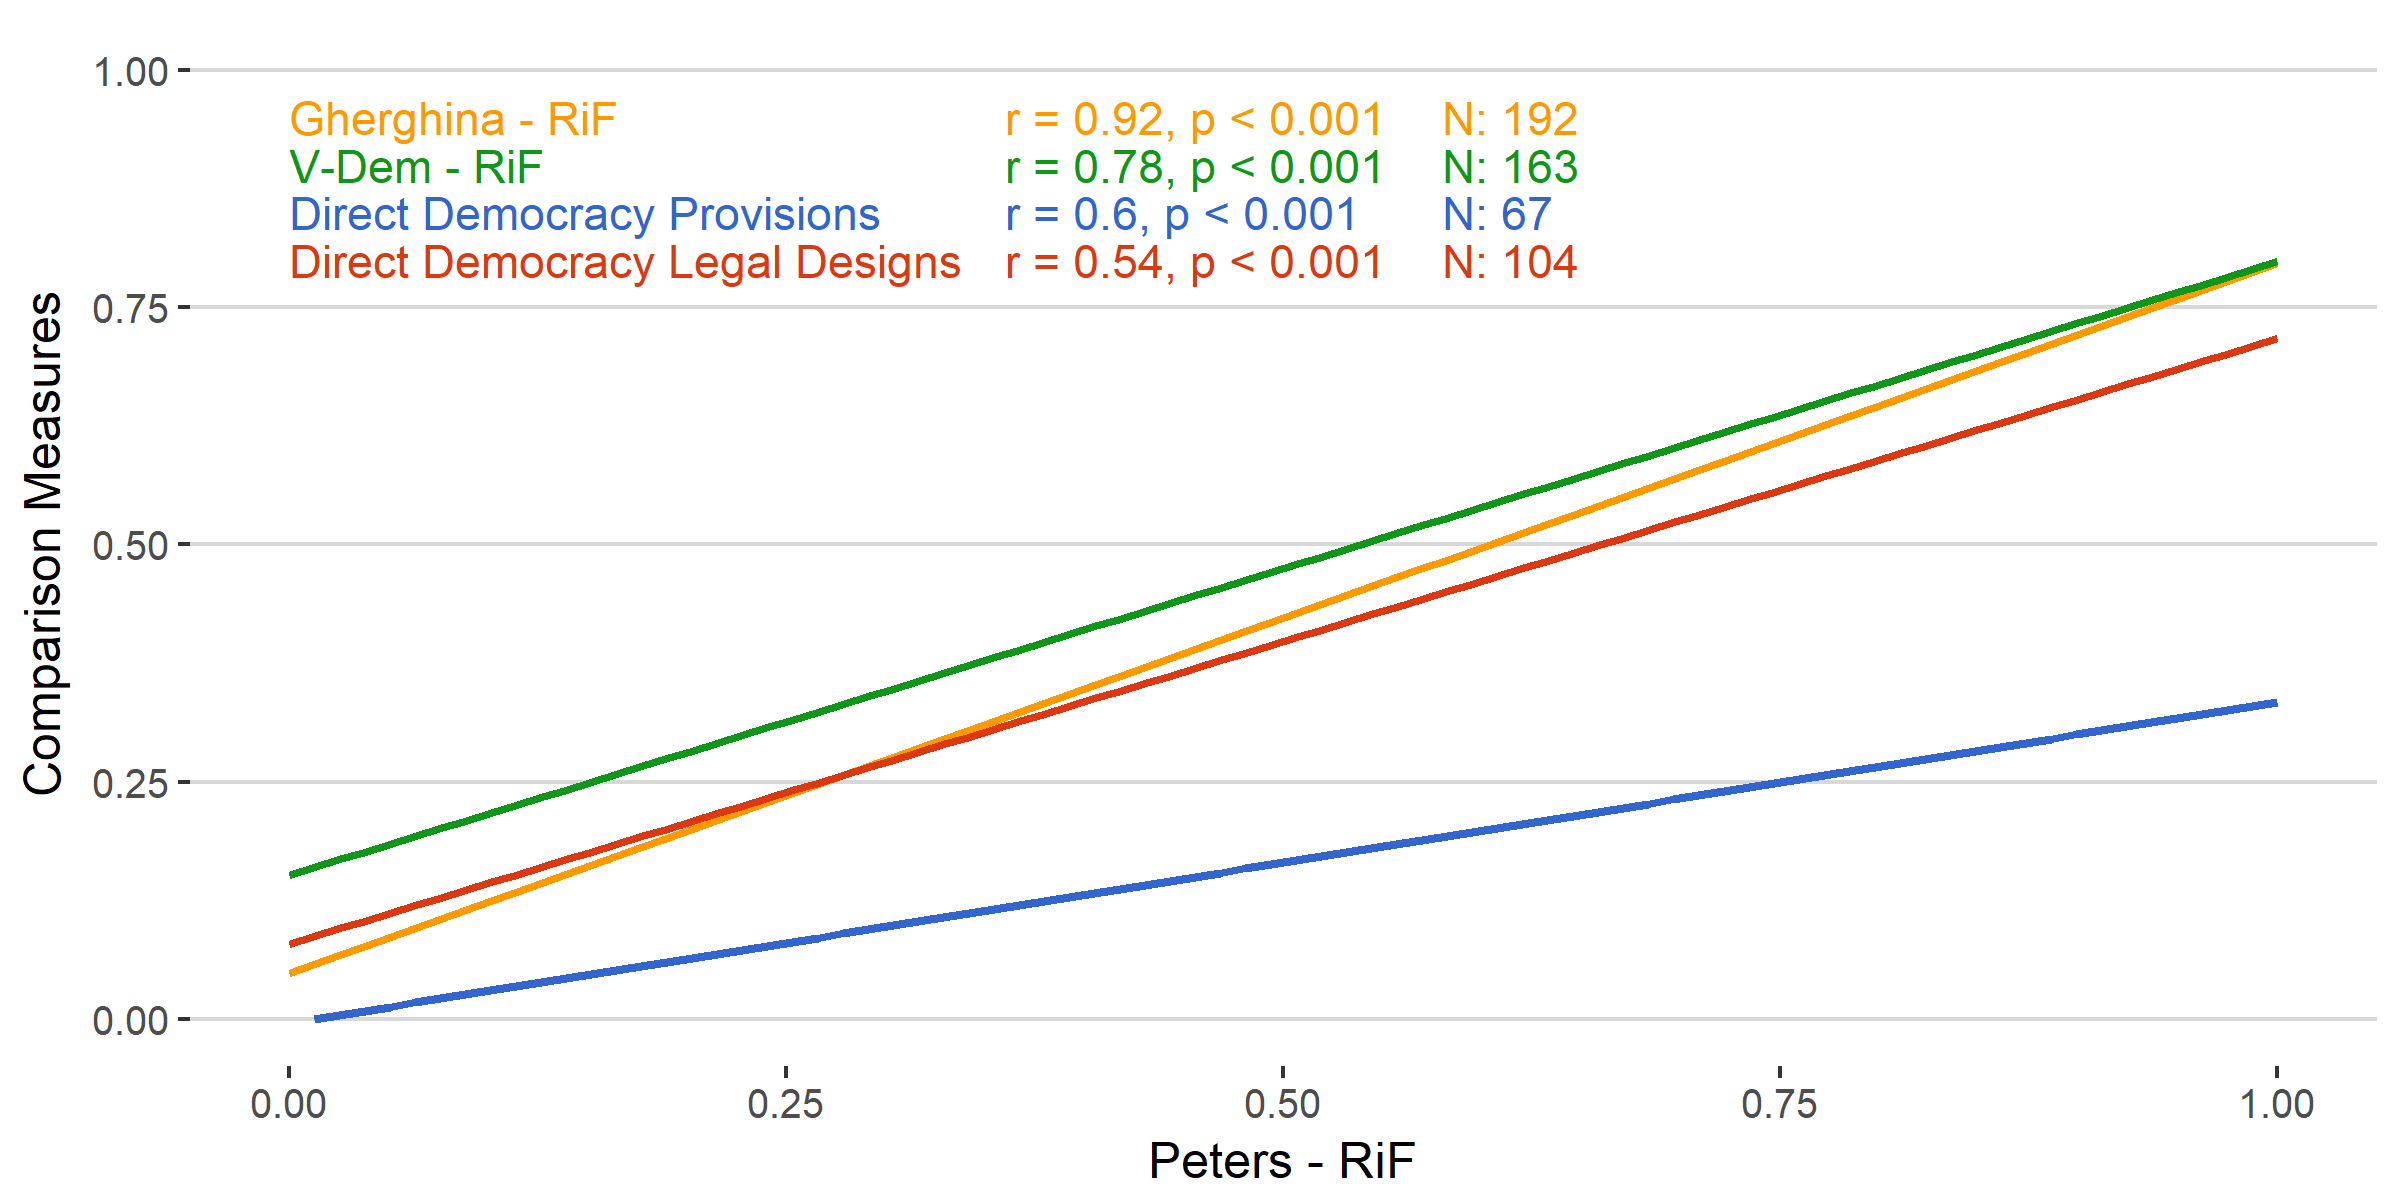
\includegraphics[width=\textwidth]{images/rif_peters.png}
    \flushright
    {\scriptsize Data sources: IDEA (2018), M. Coppedge et al. (2017), Navigator (2018b), Barometer (2016).\par}
\end{figure}

To get a better overview in regard to how the indices differ across
regime types, we compare their distributions visualized with density
plots (Figure \ref{rif_fh}), grouped according to the Freedom House
classification into free, partly free and not free countries {[}for the
construction of the Freedom House index and the classification see
@fh2018freedom{]}. It has to be noted that the visualized distributions
are rather smooth, though in case of discrete variables the original
categories can be recognized at the peaks. Most of the rules in form
measures are rather normally distributed, with many countries reaching
medium scores and few countries with high and low scores. Concerning not
free countries (if available), the distributions become more skewed,
with less countries having higher values, a pattern which appears with
all of the applicable measures. It becomes visible that the simple count
variable of Legal Designs is not very accurate, as on average even less
countries score on higher values. In general, partly free countries
score as high or even higher as the ones categorized as free on all
indicators. This implicates that the previously discussed importance of
the level of democracy should not be neglected when comparing direct
democracy across a wider range of countries. One might argue that, given
equal direct popular vote mechanisms, a semi-democratic country is still
less direct \emph{democratic}, than a ``full'' democracy. Nevertheless,
this pattern is a noteworthy discovery that should be investigated
further by future research.

\begin{figure}[!bh]
    \caption{Rules in Form Measures by Freedom House Index}
    \label{rif_fh}
    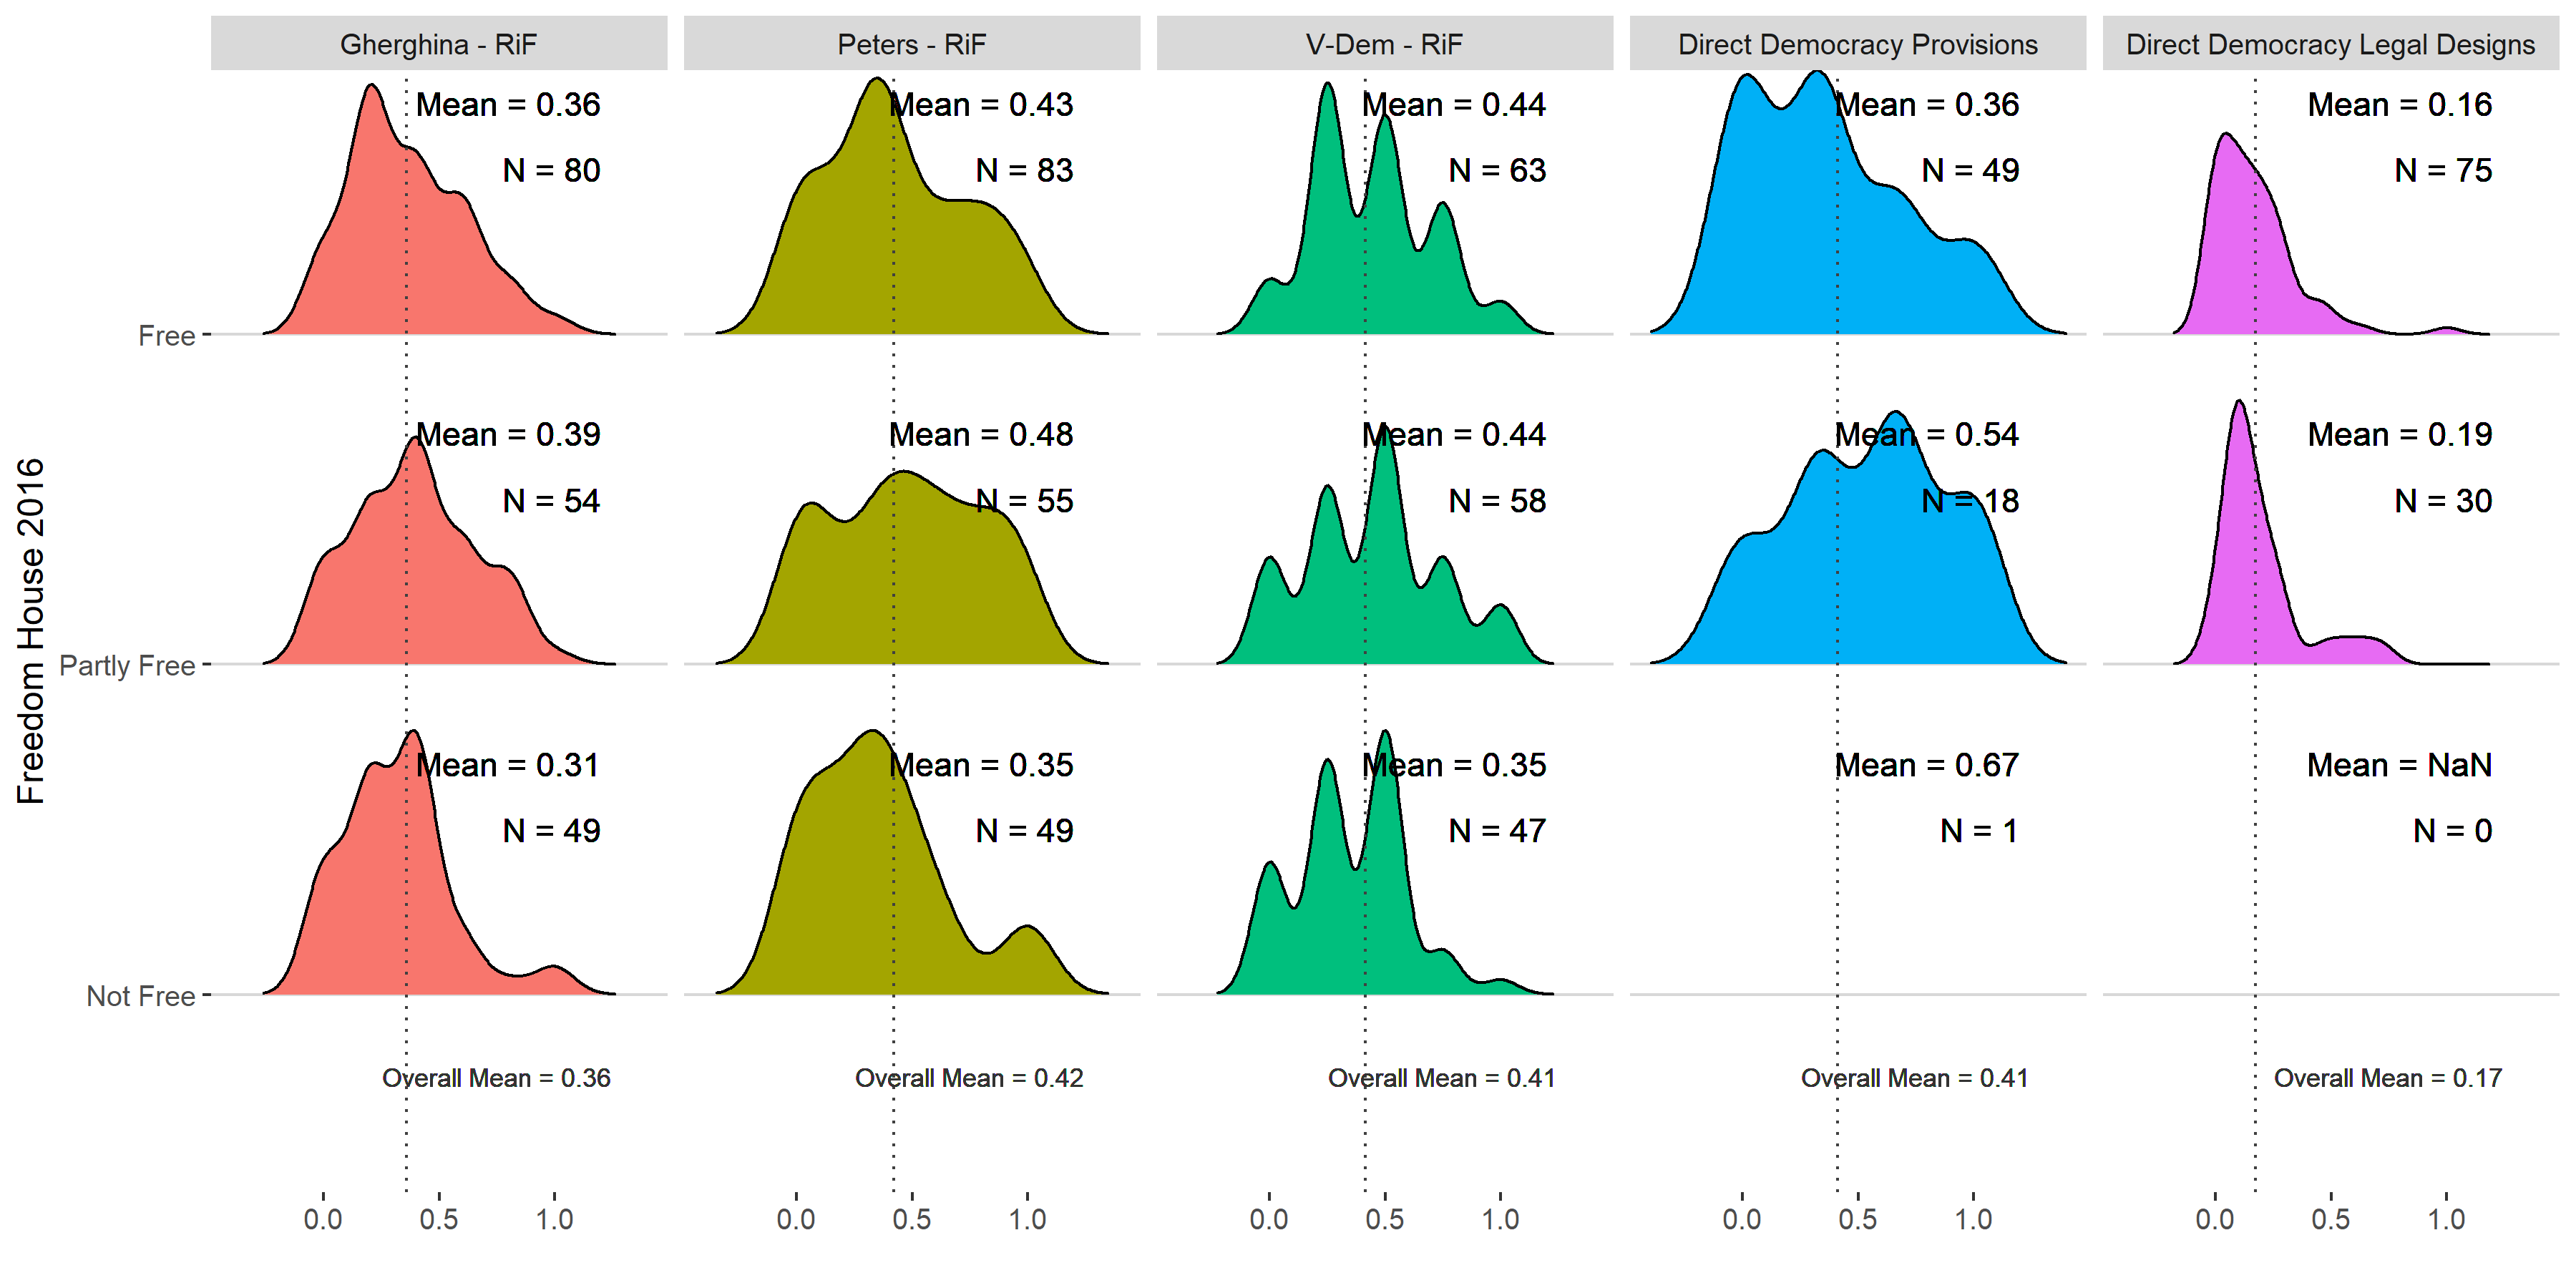
\includegraphics[width=\textwidth]{images/coef_rif2.png}
    \flushright
    {\scriptsize Data sources: IDEA (2018), M. Coppedge et al. (2017), Navigator (2018b), Barometer (2016), Freedom House (2018). \par}
\end{figure}

Next, the distributions for the two bottom-up and top-down rules in form
measures are depicted separately in Figure \ref{type_rif}. Both
indicators are rather similar, as they are both constructed using V-Dem
data. It can be observed, that top-down provisions for direct democracy
(Peters RiF Mean = 0.29; V-Dem RiF Mean = 0.53) are by far more common
than citizen initiated institutions (Peters RiF Mean = 0.19; V-Dem RiF
Mean = 0.63), which was already found by @serdultwelp2012 pp.~77.

\begin{figure}[!th]
\caption{Bottom-Up and Top-Down Rules in Form Measures}
    \label{type_rif}
    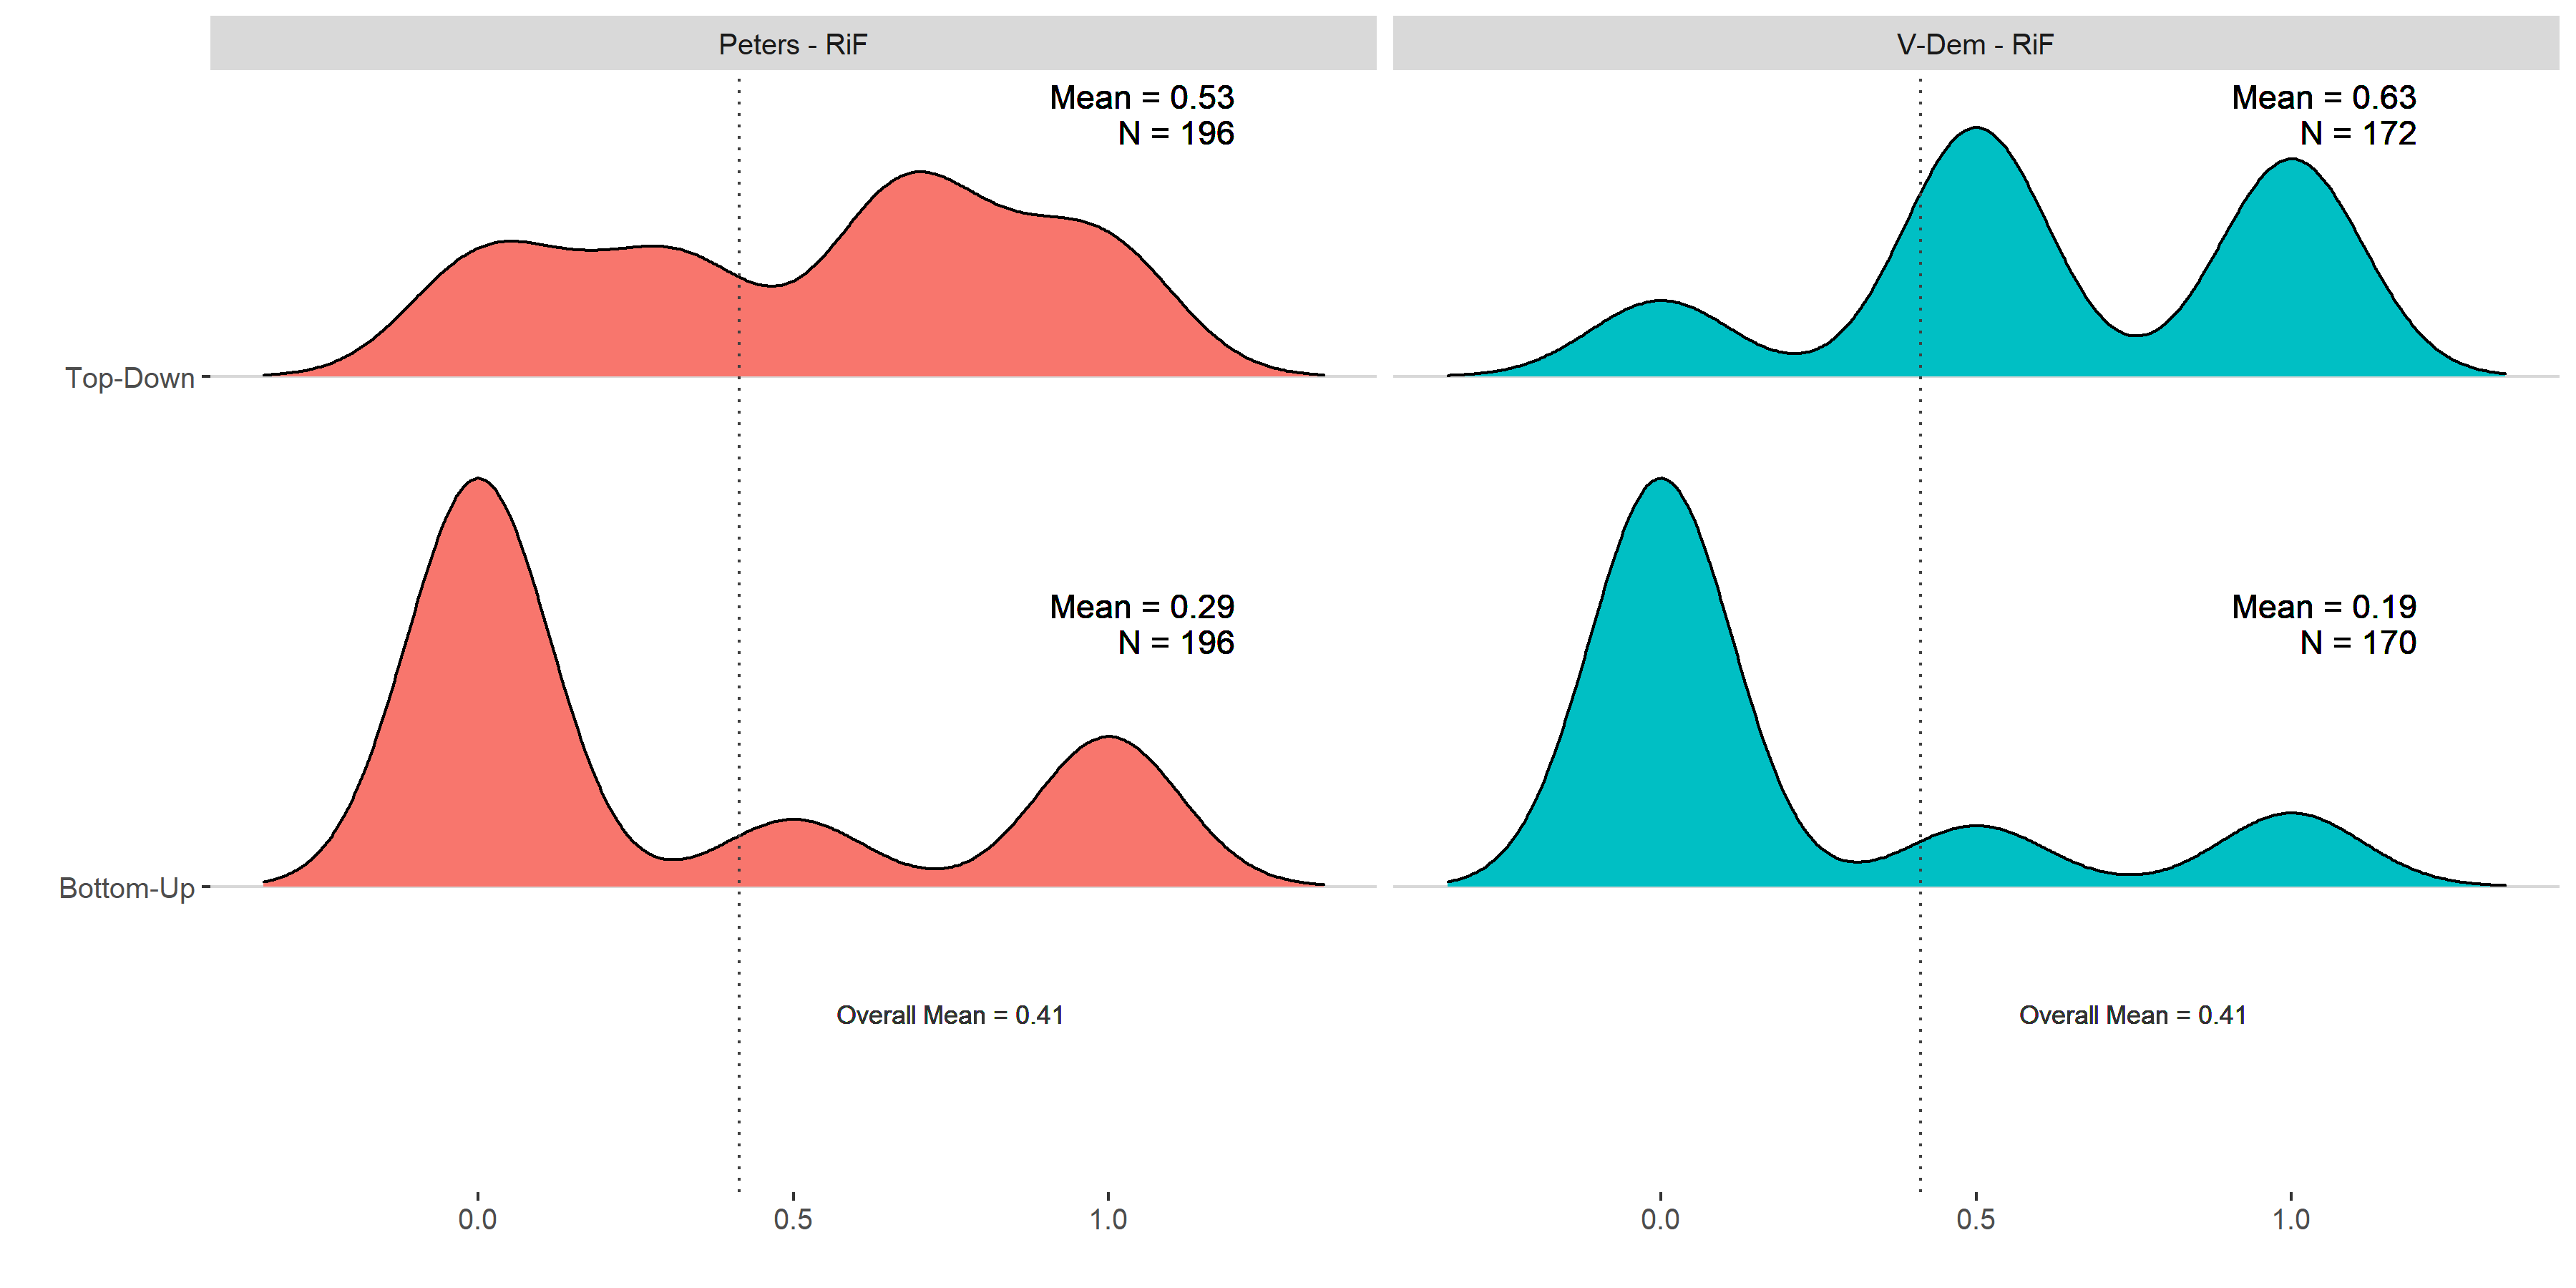
\includegraphics[width=\textwidth]{images/type_rif.png}
    \flushright
    {\scriptsize Data sources: IDEA (2018), M. Coppedge et al. (2017). \par}
\end{figure}

Figure \ref{map_rif} depicts a map, coloured according to a simple
variable, indicating whether there are provisions only for bottom-up or
top down direct democratic mechanisms, for both, or for none. Indication
of such provisions is simply an index score above 0 on the respective
measurement. Differences in classification are due to the consideration
of different mechanisms, as well as different data sources for each
measure. Here, the previous finding becomes apparent as well: a majority
of countries only provide for top-down institutions (Peters - RiF N =
95; V-Dem RiF N = 106), while, depending on the coding scheme, a much
smaller part has provisions for both (Peters - RiF N = 67; V-Dem RiF N =
42). Interestingly, those countries can be found mostly in Eastern
Europe and Latin America. There are 33 (Peters - RiF) or 24 (V-Dem -
RiF) countries that provide neither top-down nor bottom-up mechanisms.
Interestingly enough, there is a single case (the Netherlands) that has
only bottom-up mechanisms in place, as indicated by the Peters - RiF
measure.

\begin{figure}[!h]
\caption{Rules in Form Measures - World Map}
\label{map_rif}
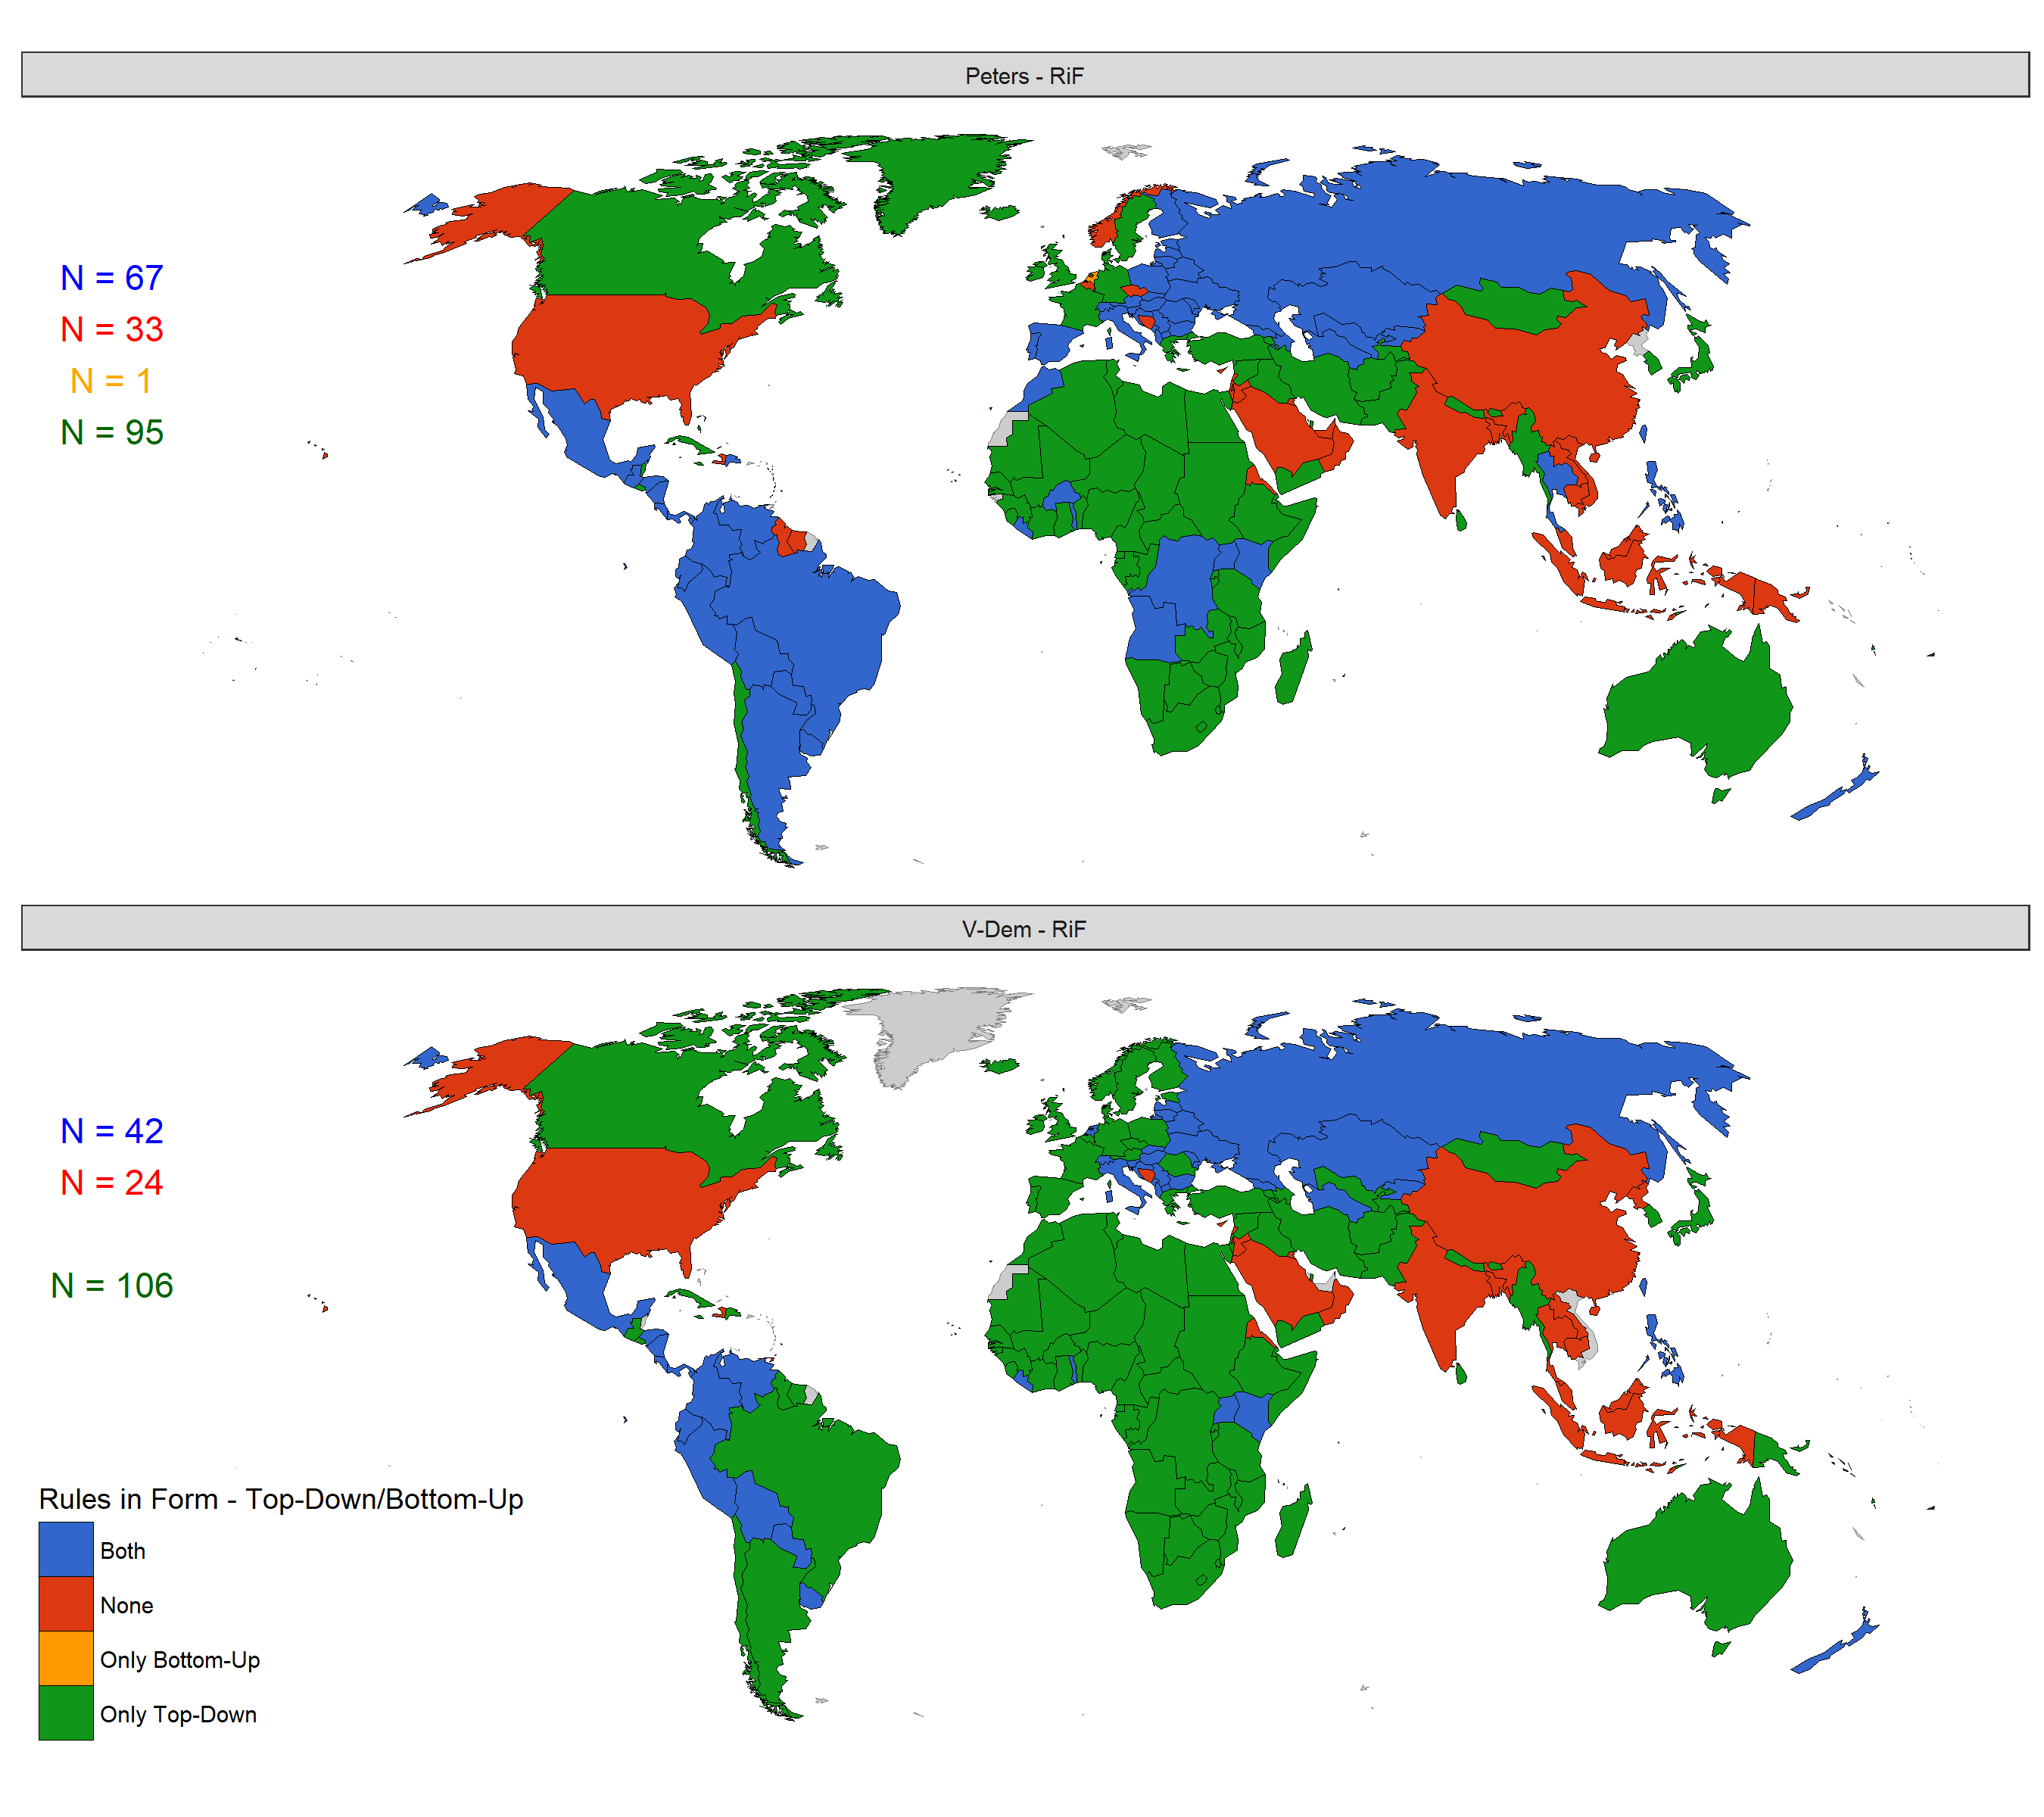
\includegraphics[width=\textwidth]{images/map_rif.png}
\flushright
    {\scriptsize Data sources: IDEA (2018), M. Coppedge et al. (2017).\par}
\end{figure}

\subsection{Comparing Rules in Use Measures} \label{riu_empiric}

As we examine even more rules in use indicators, only one approach is
compared with the others, namely Gherghina - RiU, the measure
constructed following @gherghina2016, as it differs the most in regard
to construction (easiness of approval and decisiveness are accounted
for). As most of the indices rely on some kind of count measure, and
empirically there are many countries in which direct democracy is rarely
used, but very few in which it is used extensively (the most prominent
example being Switzerland, but also Uruguay and Azerbaijan stand out as
outliers), we use the rank-based correlation coefficient Spearman's Rho
to account for the heavily skewed data.

The summed up indicator based on V-Dem data shows the strongest relation
to the Gherghina measure(Rho = 0.98), which was also constructed using
V-Dem data (Figure \ref{riu_ghergina}). All the other indicators have
strong correlations as well, the least being the Effective Use count
measure (Rho = 0.65). In average, the indices seem to be in line with
the Gherghina - RiU, although the Sudd - RiU Sum as well as the Credible
Use indicators are systematically observed at higher values.

\begin{figure}[!th]
    \caption{Gherghina RiU compared to other Rules in Use Measures}
    \label{riu_ghergina}
    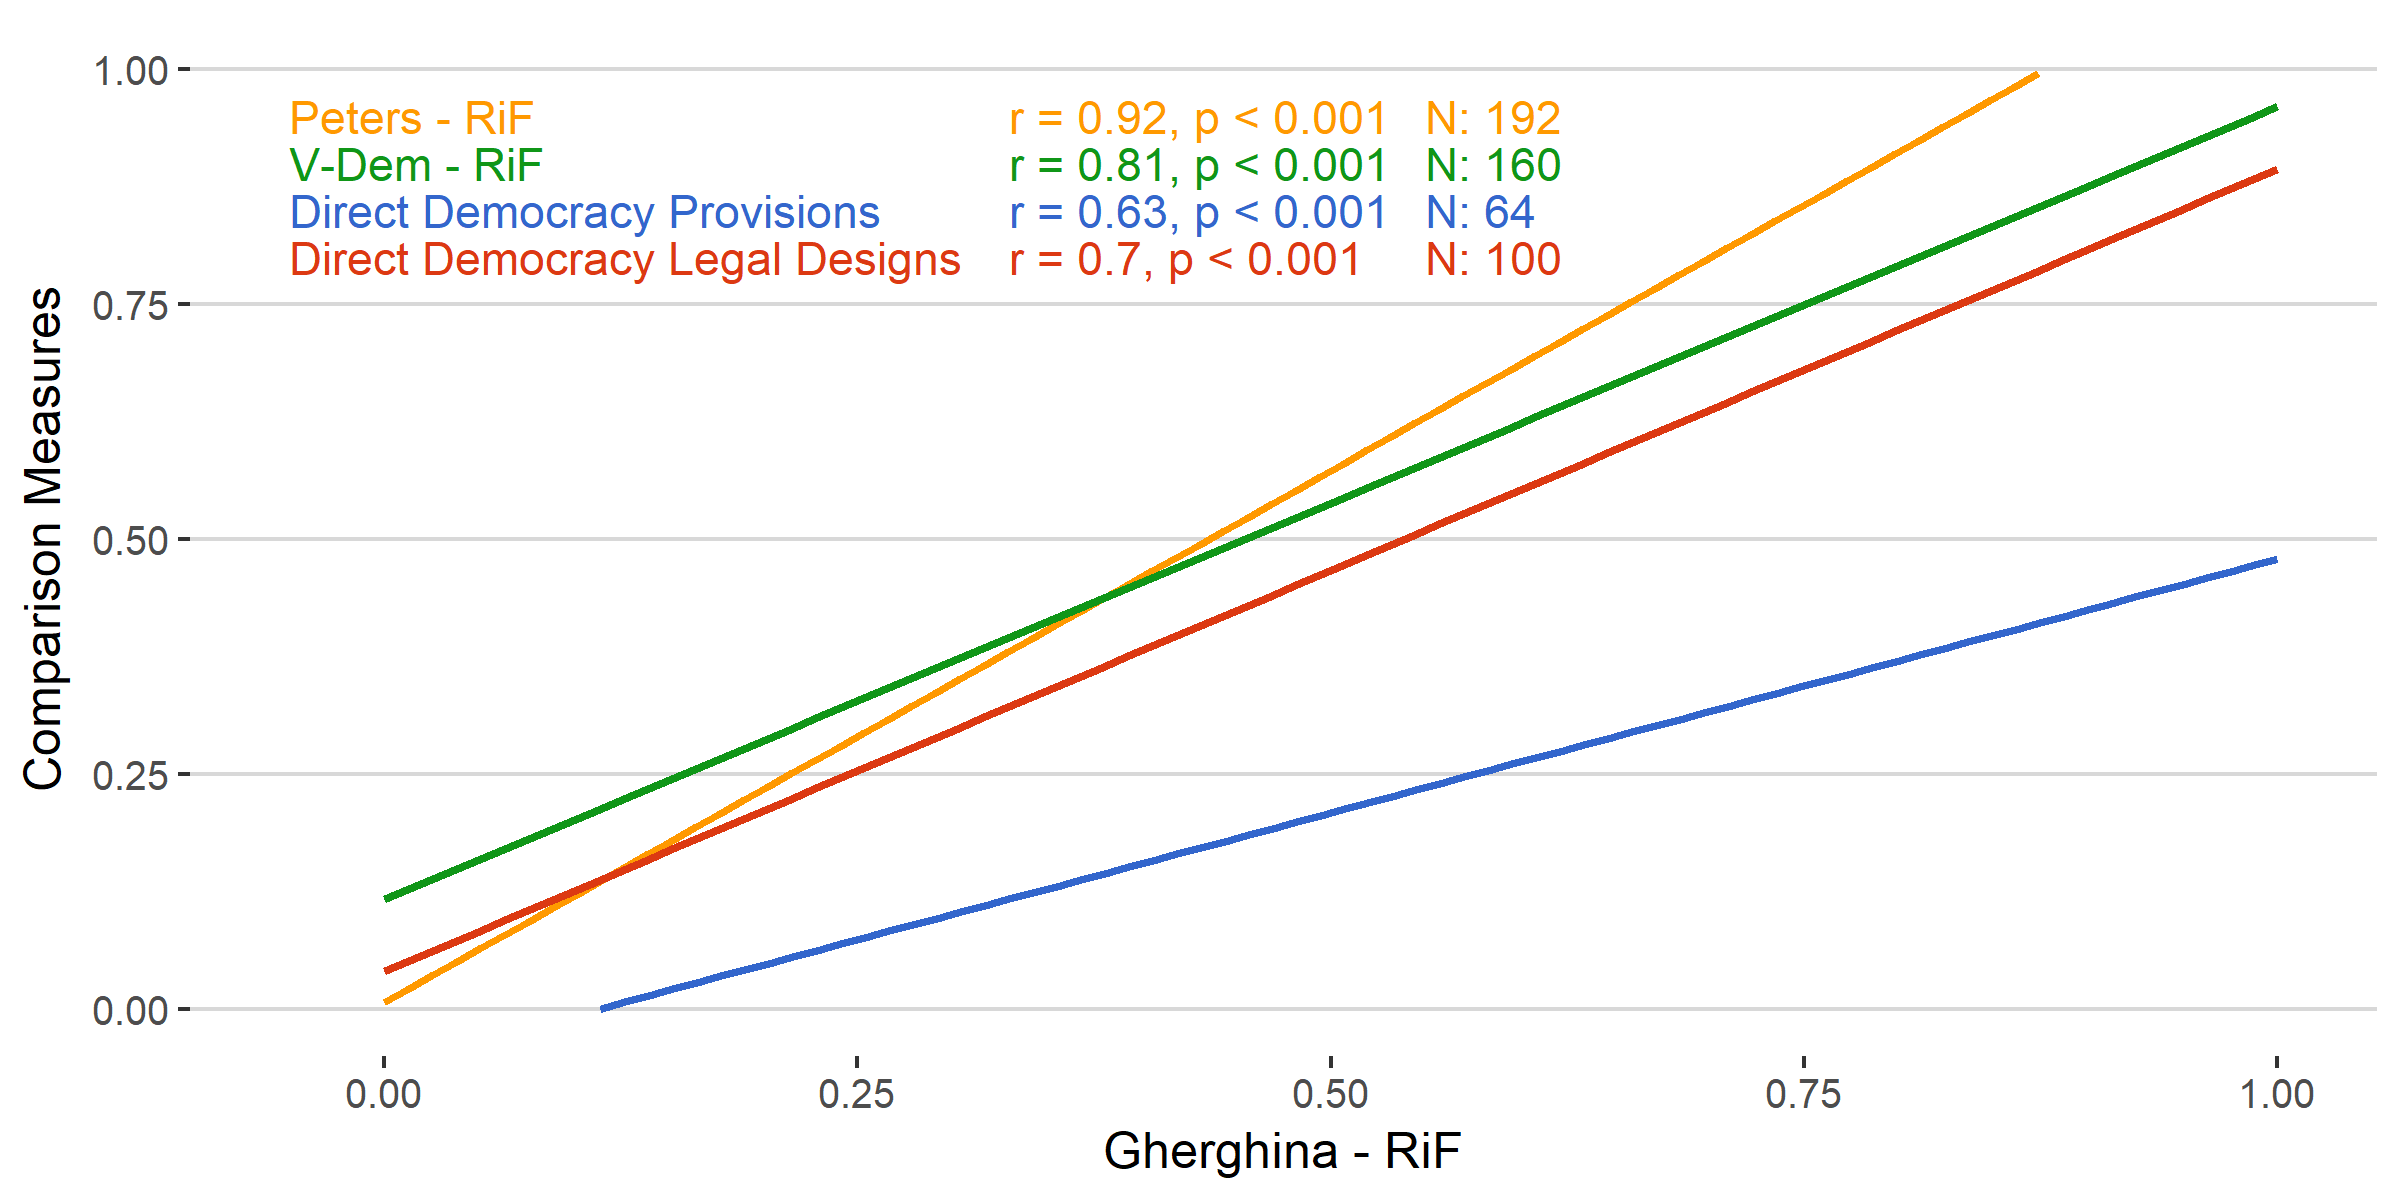
\includegraphics[width=\textwidth]{images/rif_ghergina.png}
    \flushright
    {\scriptsize Based on own calculations. \par}
\end{figure}

riu\_ghergina

Figure \ref{coef_riu2} depicts the distributions for the rules in use
indicators, for which it can be observed that the summed up indicators,
and also the Gherghina - RiU measure are heavily skewed, with very few
countries ranging very high, while most are located at the lowest
scores. Due to construction, this does not apply as much to the Credible
Use indicator, and even less to the categorical classifications,
illustrating an important advantage of such measurement approaches, even
if it implies a loss of empirical information.

\begin{figure}[!th]
    \caption{Rules in Form Measures by Freedom House Index}
    \label{coef_riu2}
    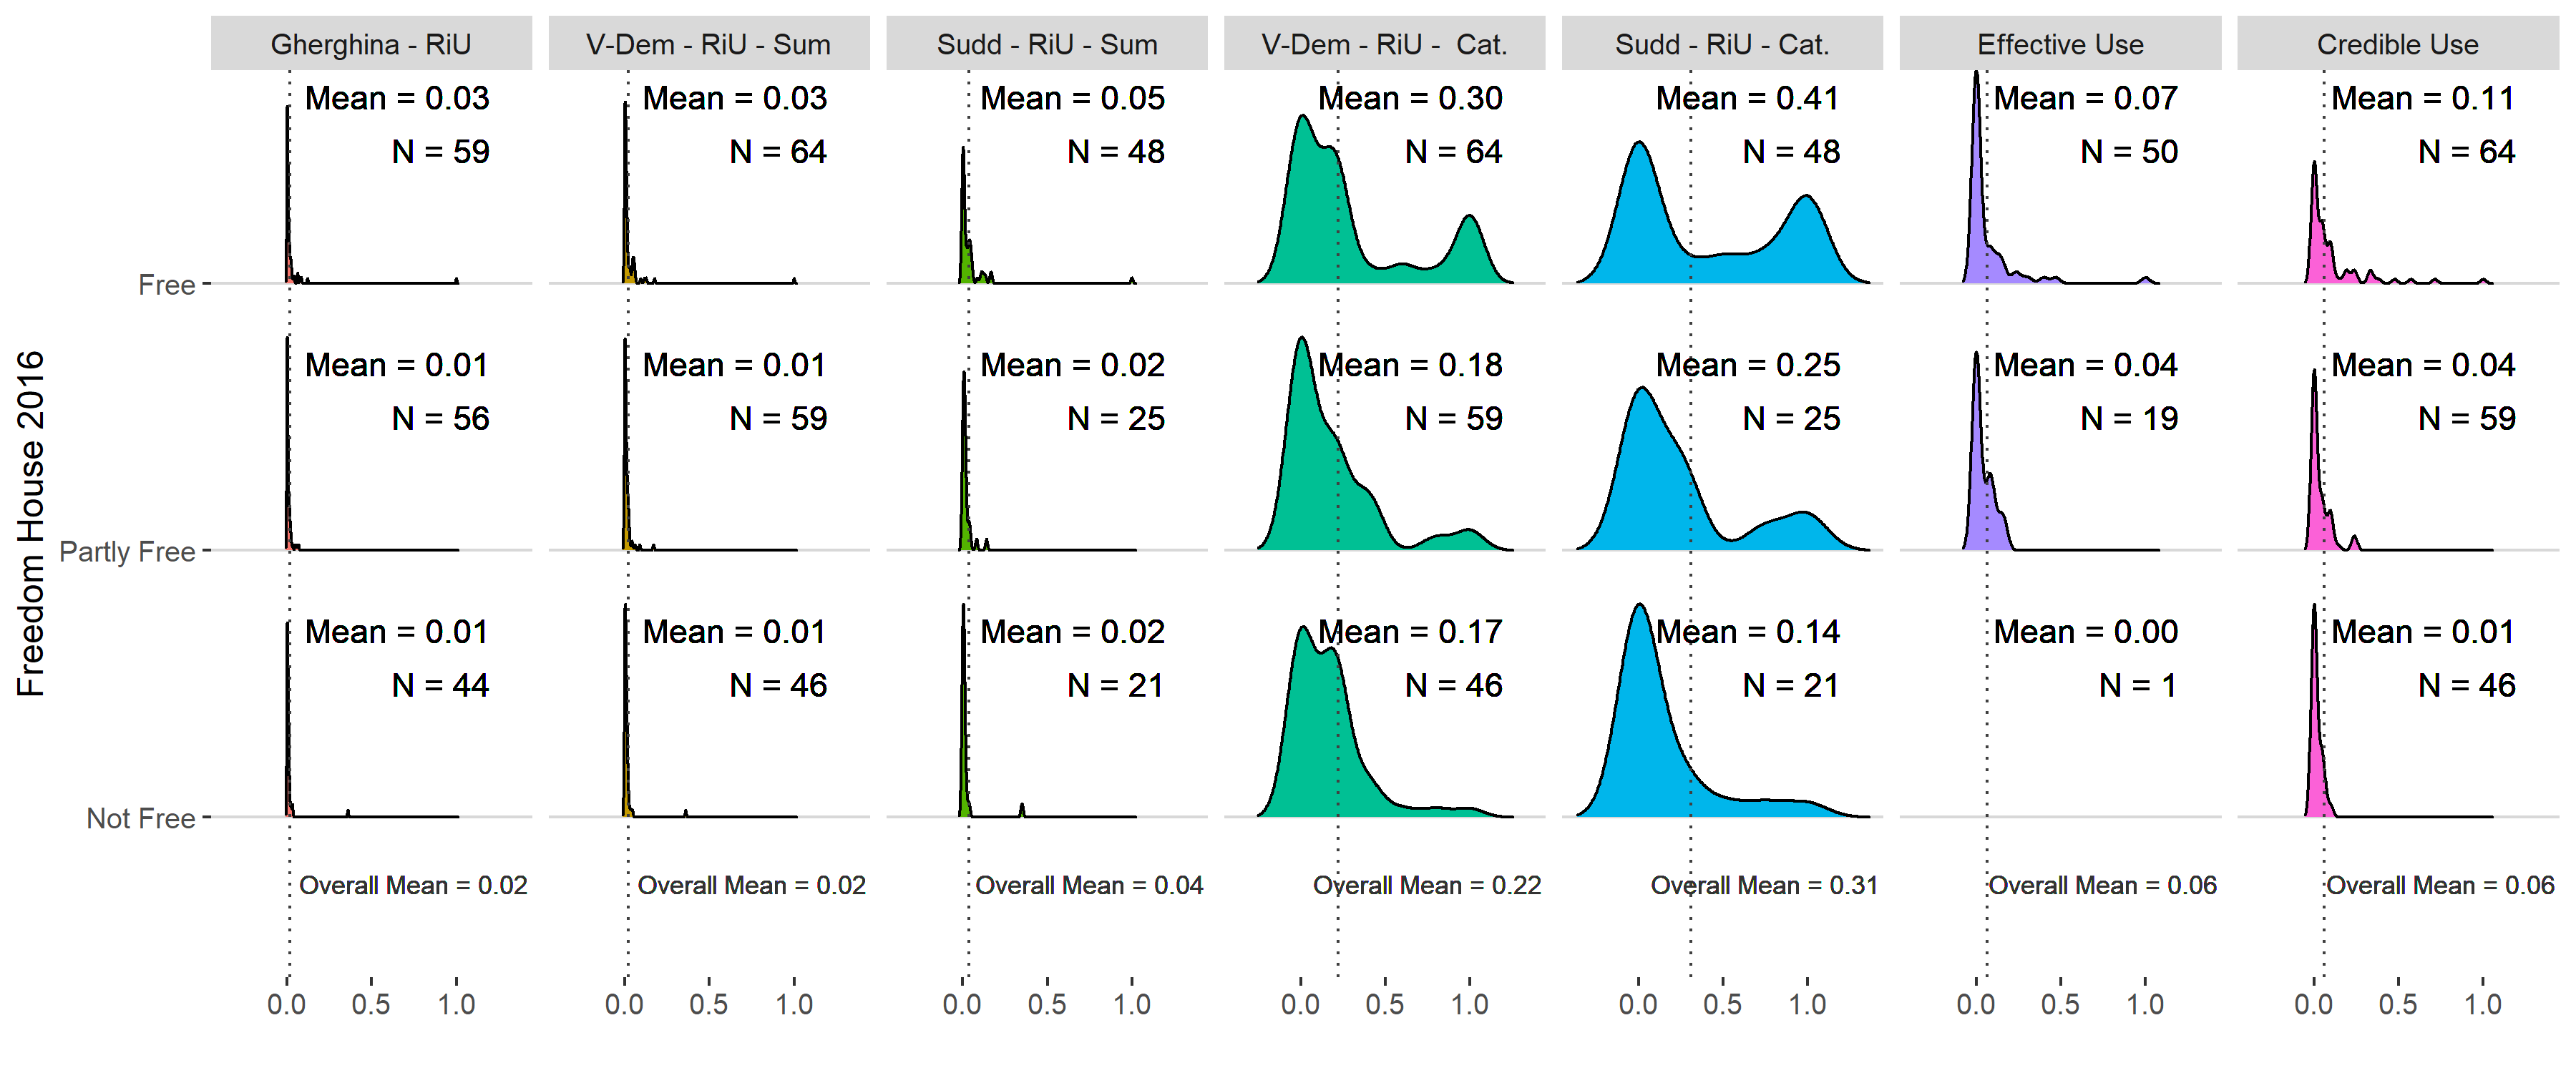
\includegraphics[width=\textwidth]{images/coef_riu2.png}
    \flushright
    {\scriptsize Based on own calculations. \par}
\end{figure}

coef\_riu2

In Figure \ref{type_riu}, the categorial variables for top-down and
bottom-up rules in use are depicted. For the V-Dem - RiU Categorized
measure, it is evident that mostly top-down mechanisms are used in
practice (Mean = 0.19) , while bottom-up mechanisms remain mainly unused
(Mean = 0.05), wich was also observed by @serdultwelp2012 pp.~78. Of
course, this is partially due to the fact that top-down mechanisms are
much less common as rules in form, and citizens can't use bottom-up
mechanisms if they are not provided. On the contrary, the Sudd - RiU
Categorized measure implies an opposite trend: bottom-up usage has a
mean of 0.40, while top-down usage has a mean of 0.24. However, this
discrepancy arises from the structure of the sudd data, that only
records direct democracy mechanisms that actually occurred. Correctly
interpreted it can be said fewer bottom-up measures have taken place (N
= 23) compared to top-down measures (N = 92).

\begin{figure}[!th]
    \caption{Bottom-Up and Top-Down Rules in Form Measures}
    \label{type_riu}
    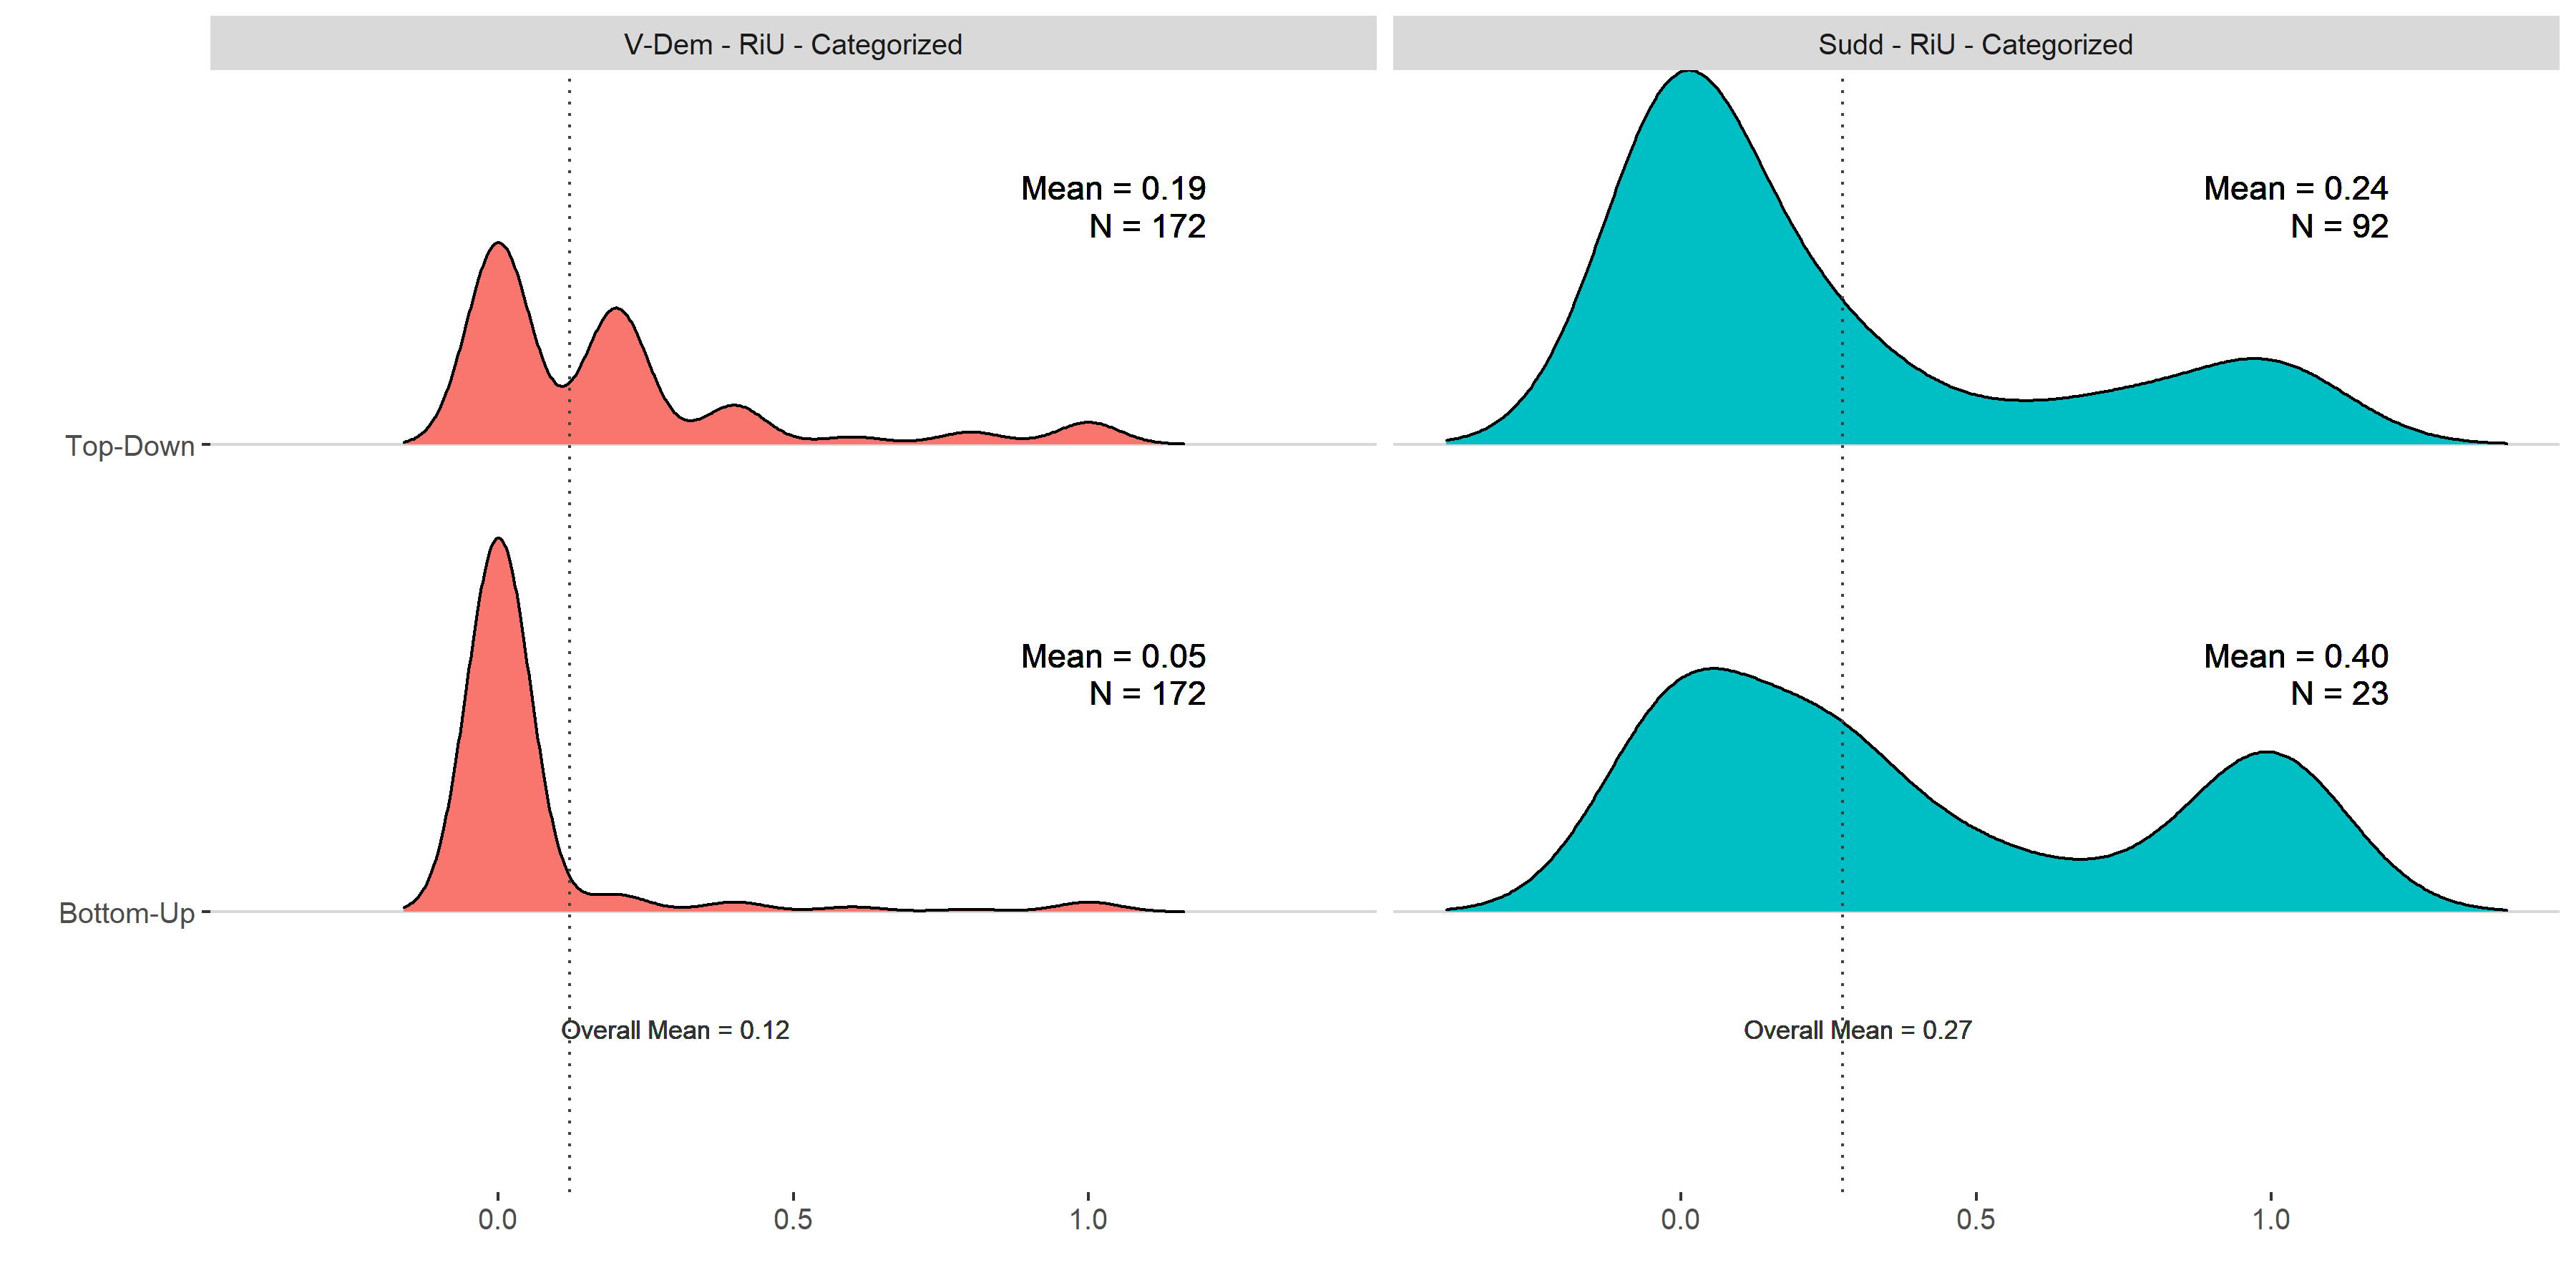
\includegraphics[width=\textwidth]{images/type_riu.png}
    \flushright
    {\scriptsize Based on own calculations. \par}
\end{figure}

type\_riu

Similar to the map depicting rules in form, Figure \ref{map_riu} depicts
a world map indicating whether, a country had at least one occurrence of
only top-down or bottom up direct popular votes in between 1996 and
2016, or whether both occured at least once. As discussed before, the
sudd dataset only embodies countries with at least one occurrence, which
becomes obvious in comparison with the V-Dem measure. Most countries are
assigned to the same category, for example both measures show that
Ukraine, Macedonia and Peru are the three countries where only bottom-up
measures occured. A few exceptions can also be noted, for example
Bolivia, which had only a top-down occurrence according to sudd, while
V-Dem counts both top-down and bottom-up rules in use. In line with the
previously described results, the biggest group consists of countries
that used neither bottom-up nor top-down direct democracy (V-Dem - RiU N
= 80), following such countries in which only top-down mechanisms are
used (Sudd - RiU N = 72; V-Dem - RiU N = 74). Countries in which both
mechanisms were used (Sudd - RiU N = 20; V-Dem - RiU N = 15) are mostly
centered in Europe, while in Africa and Latin America mostly top-down
mechanisms are practiced exclusively (which is not very surprising, as
many countries in this regions only provide for such mechanisms).

\begin{figure}[!th]
    \caption{Rules in Use Measures - World Map}
    \label{map_riu}
    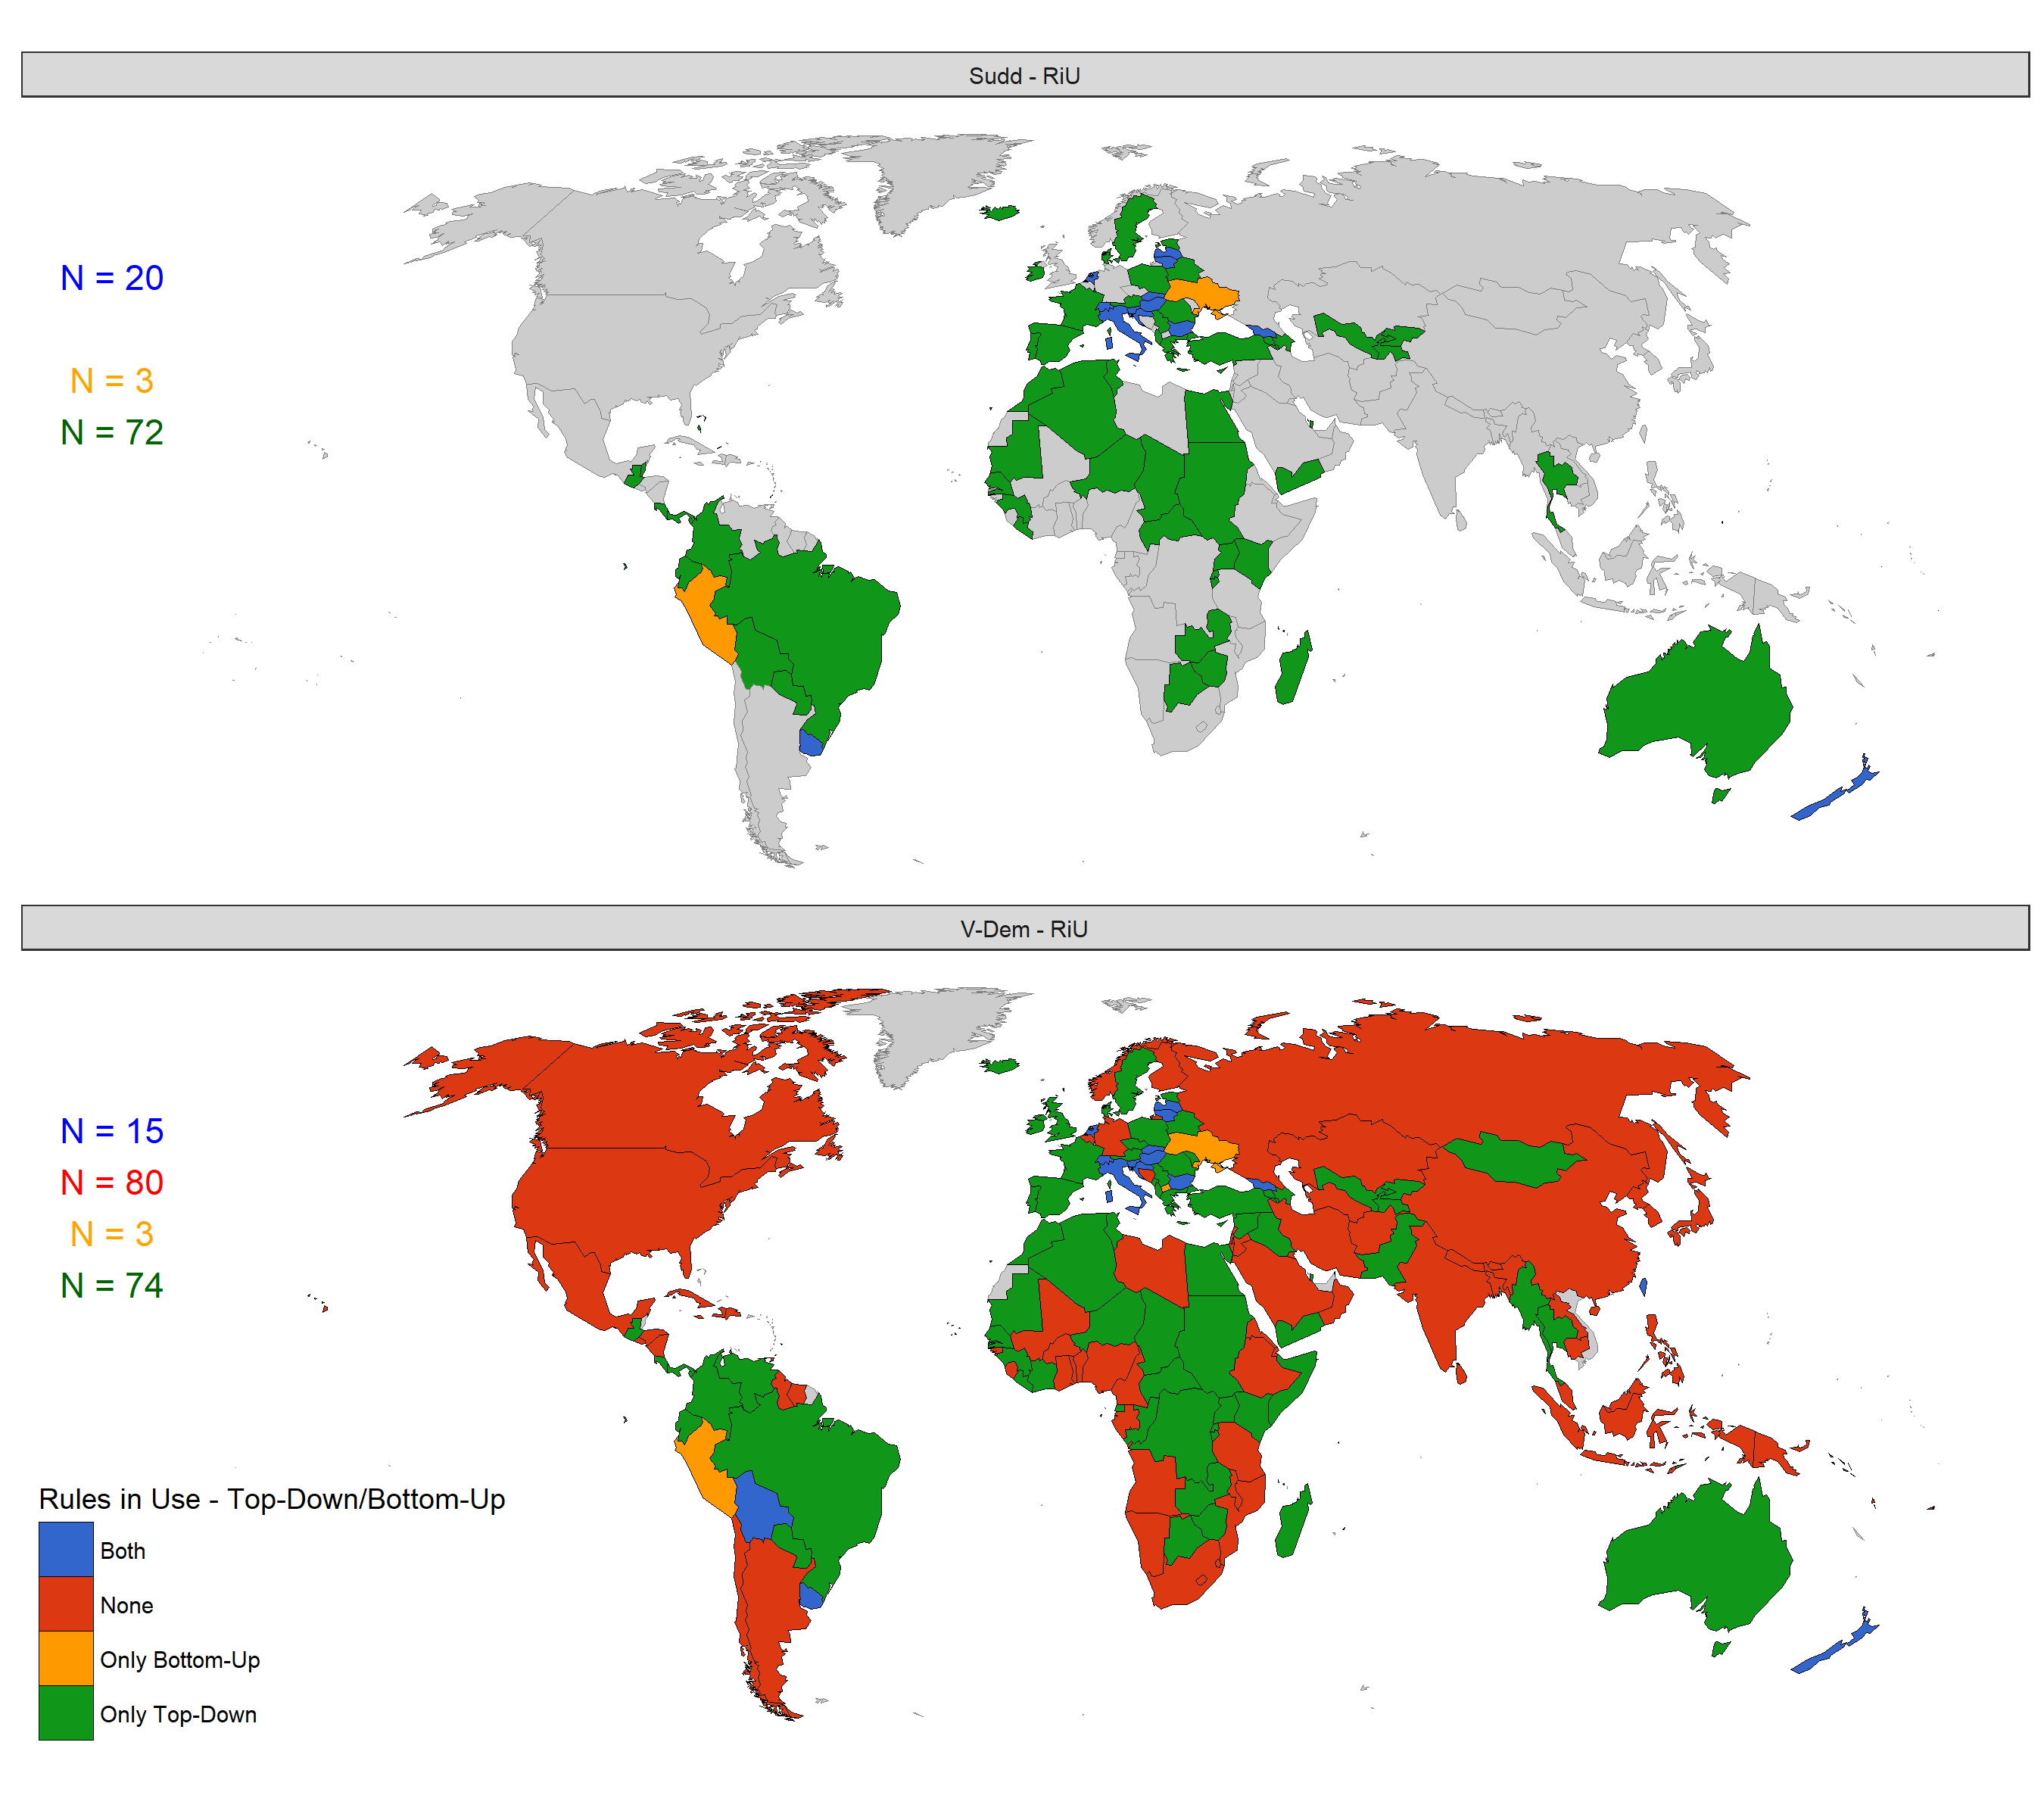
\includegraphics[width=\textwidth]{images/map_riu.png}
    \flushright
    {\scriptsize Based on own calculations. \par}
\end{figure}

map\_riu

\subsection{Comparing Mixed Measures} \label{mixed_empiric}

As we are only assessing two mixed measurement approaches, we compare
them in a more detailed way. Figure \ref{mixed} depicts a scatterplot of
Fiorinos Direct Democracy Index and the Direct Popular Vote Index from
Altman/V-Dem. It becomes visible, that the Fiorino Idex also considers
the general level of democracy, while the other measure only accounts
for the direct popular vote dimension. For example, countries like the
Ukraine or Venezuela score high on the DPVI, but not on the Direct
Democracy Index. In general, there are more countries that get
relatively higher scores in the @fiorino2017 measure than the DPVI, for
example the Netherlands, Philippines or Belgium. As both indices capture
a wide range of variables, and the DPVI is aggregated in a complex
fashion while the Direct Democracy Index is a qualitative assessment,
diverging scores are not very surprising. In regard to the Freedom House
classification, countries labeled as free score higher on average on the
Direct Democracy Index than countries of the other two Freedom House
categories (see Figure \ref{boxplots_final}). As expected, the DPVI
shows no such pattern. In contrary, the median is highest for the
countries categorized as not free, though it has to be noted that the
boxplots only depict results for the sample available for both indices,
which means a proportionally large number of autocracies are not
considered.

\begin{figure}[!th]
    \caption{Scatterplot - DDi vs. DPVI}
    \label{mixed}
    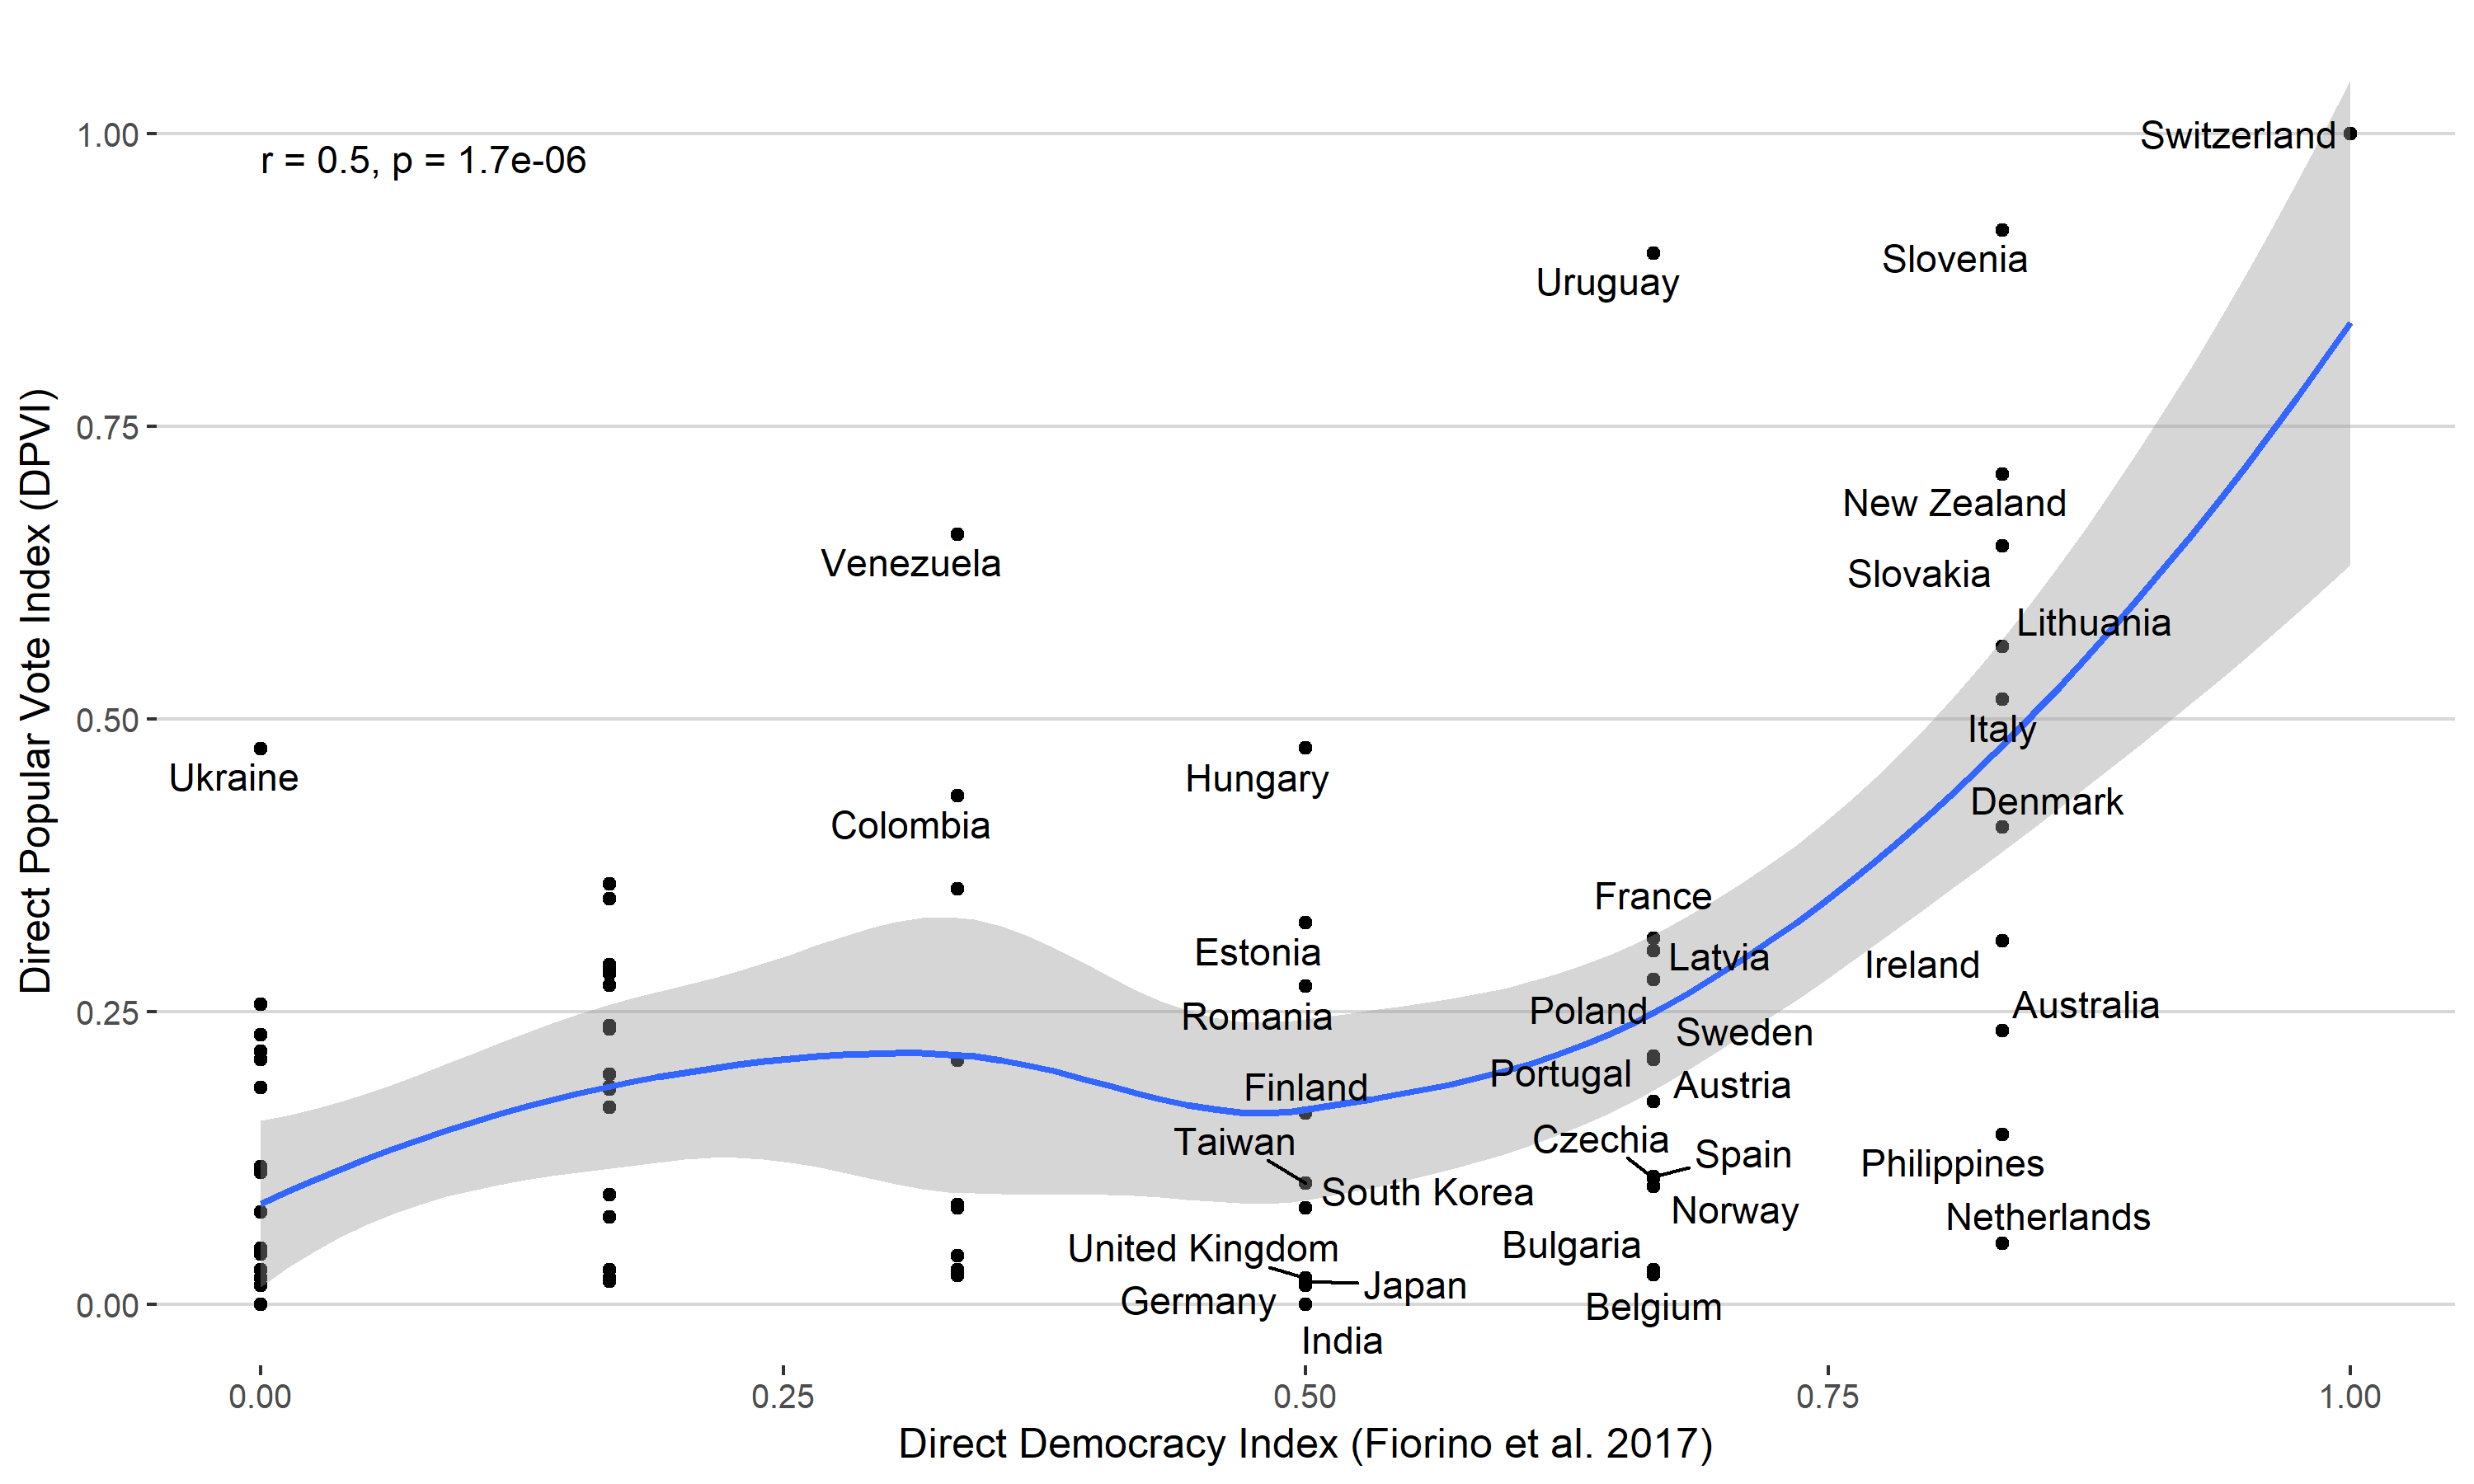
\includegraphics[width=\textwidth]{images/mixed.png}
    \flushright
    {\scriptsize Based on own calculations. \par}
\end{figure}

\begin{figure}[!th]
    \caption{Mixed Measures by Freedom House Index}
    \label{boxplots_final}
    \includegraphics[width=\textwidth]{images/boxplots_final.png}
    \flushright
    {\scriptsize DDI: Not Free = 16, Partly Free = 22, Free = 49; DPVI: Not Free = 44, Partly Free = 56, Free = 67; Based on own calculations. \par}
\end{figure}

mixed boxplots\_final Annotations: N,

World maps for both the DDI and the DPVI are depicted in Figures
\ref{map_fiorini_fin} and \ref{map_altmann_fin} respectively. The
Fiorino measure indicate high levels of direct democracy especially in
Europe (and Australia), while the pattern for the DPVI is quite
different. Here, only few countries stand out with high values (for
example Switzerland, Uruguay, Venezuela), while Central Europe is shaded
darker than in the Fiorino map. So, once again, it becomes visible that
only the Fiorino index considers the general level of democracy.

\begin{figure}[!th]
    \caption{Direct Democracy Index - World Map}
    \label{map_fiorini_fin}
    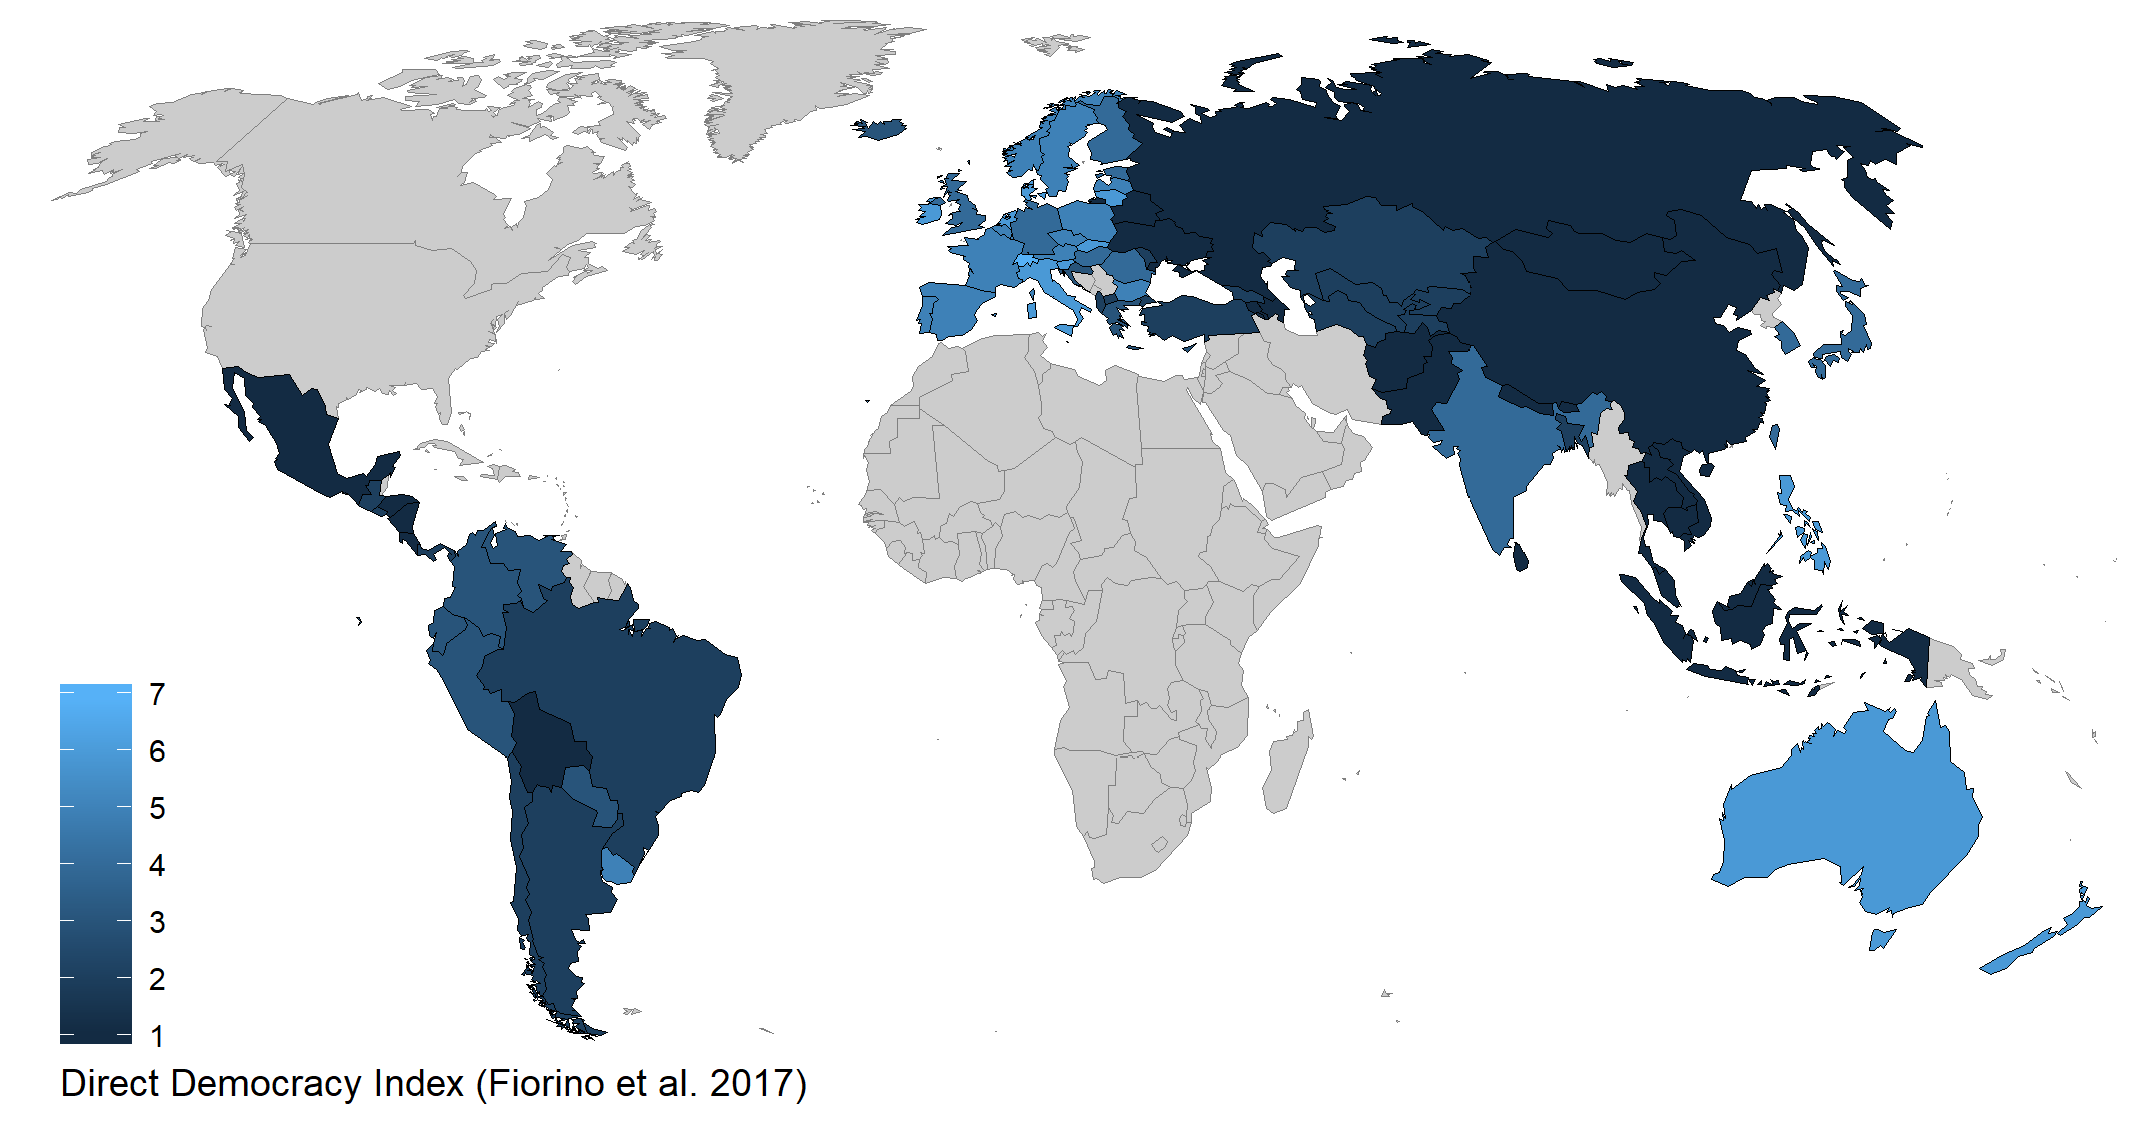
\includegraphics[width=\textwidth]{images/map_fiorini_fin.png}
    \flushright
    {\scriptsize Based on own calculations. \par}
\end{figure}\begin{figure}[!th]
    \caption{Direct Popular Vote Index - World Map}
    \label{map_altmann_fin}
    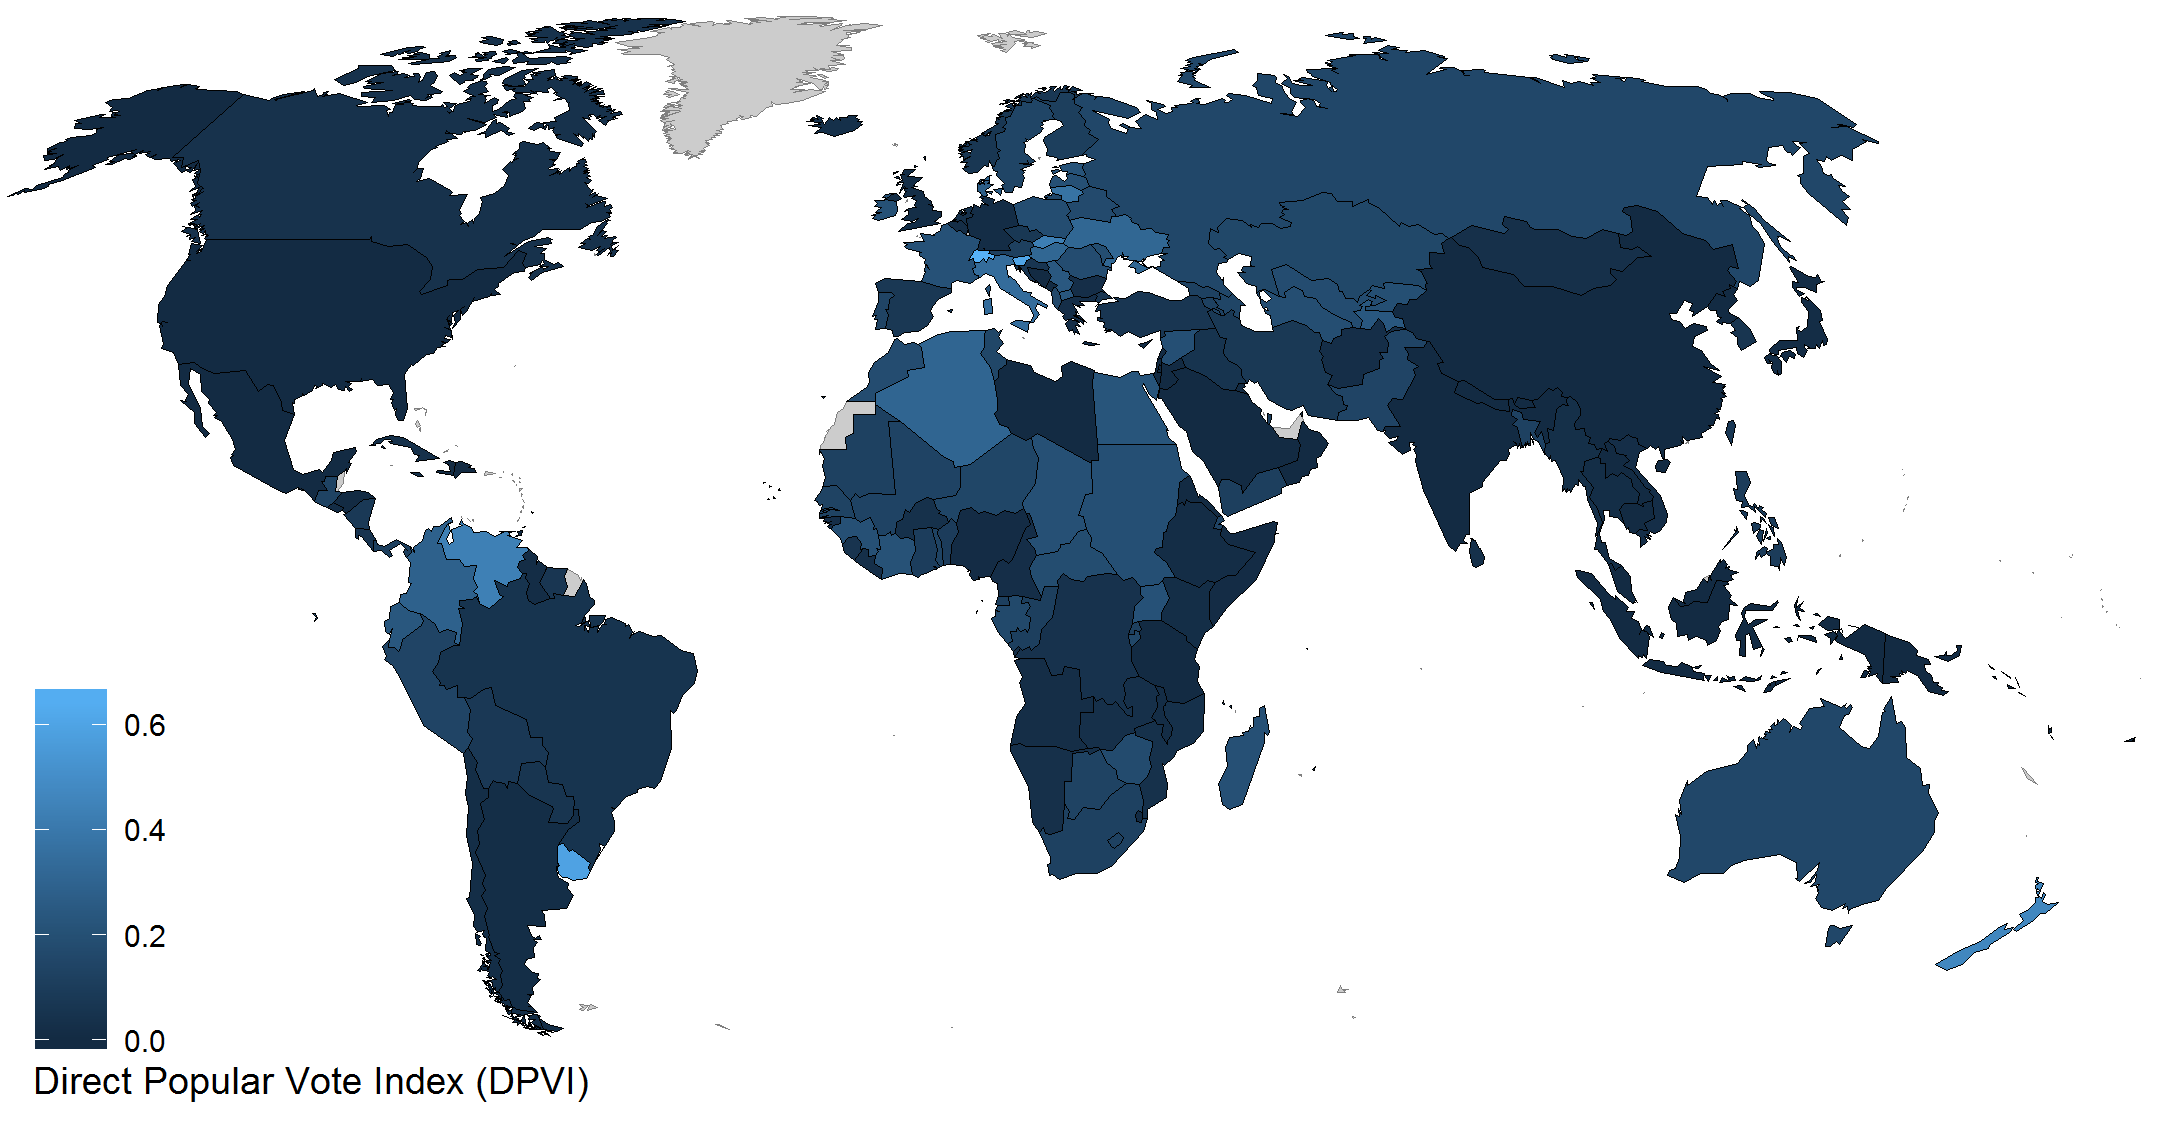
\includegraphics[width=\textwidth]{images/map_altmann_fin.png}
    \flushright
    {\scriptsize Based on own calculations. \par}
\end{figure}

map\_fiorini\_fin map\_altmann\_fin

Lastly, we take a look at the DPVI subindices for bottom-up and
top-down, as depicted in Figure \ref{altman_tpbu}. Countries scoring
high primarily on the top-down measure appear in the top-left corner,
first and foremost Venezuela, but for example also Algeria, Denmark and
Tajikistan. The countries with the highest levels of bottom-up direct
popular votes are Slovenia, Switzerland and Uruguay. Comparatively low
levels of top-down but high levels of bottom-up direct popular votes can
be found for example in Latvia, Georgia and Ukraine. In general, it
becomes visible that direct democratic institutions are primarily common
in their top-down variant, with only a small number of countries scoring
high on the bottom-up sub-index, and most countries having scores of
zero. A correlation between the two measures implies an association
between top-down and bottom-up indices, however this is mostly based on
a few outlier countries that were already discussed (r = 0.24).

altman\_tpbu

\begin{figure}[!th]
    \caption{Bottom-Up and Top-Down Components of DPVI}
    \label{altman_tpbu}
    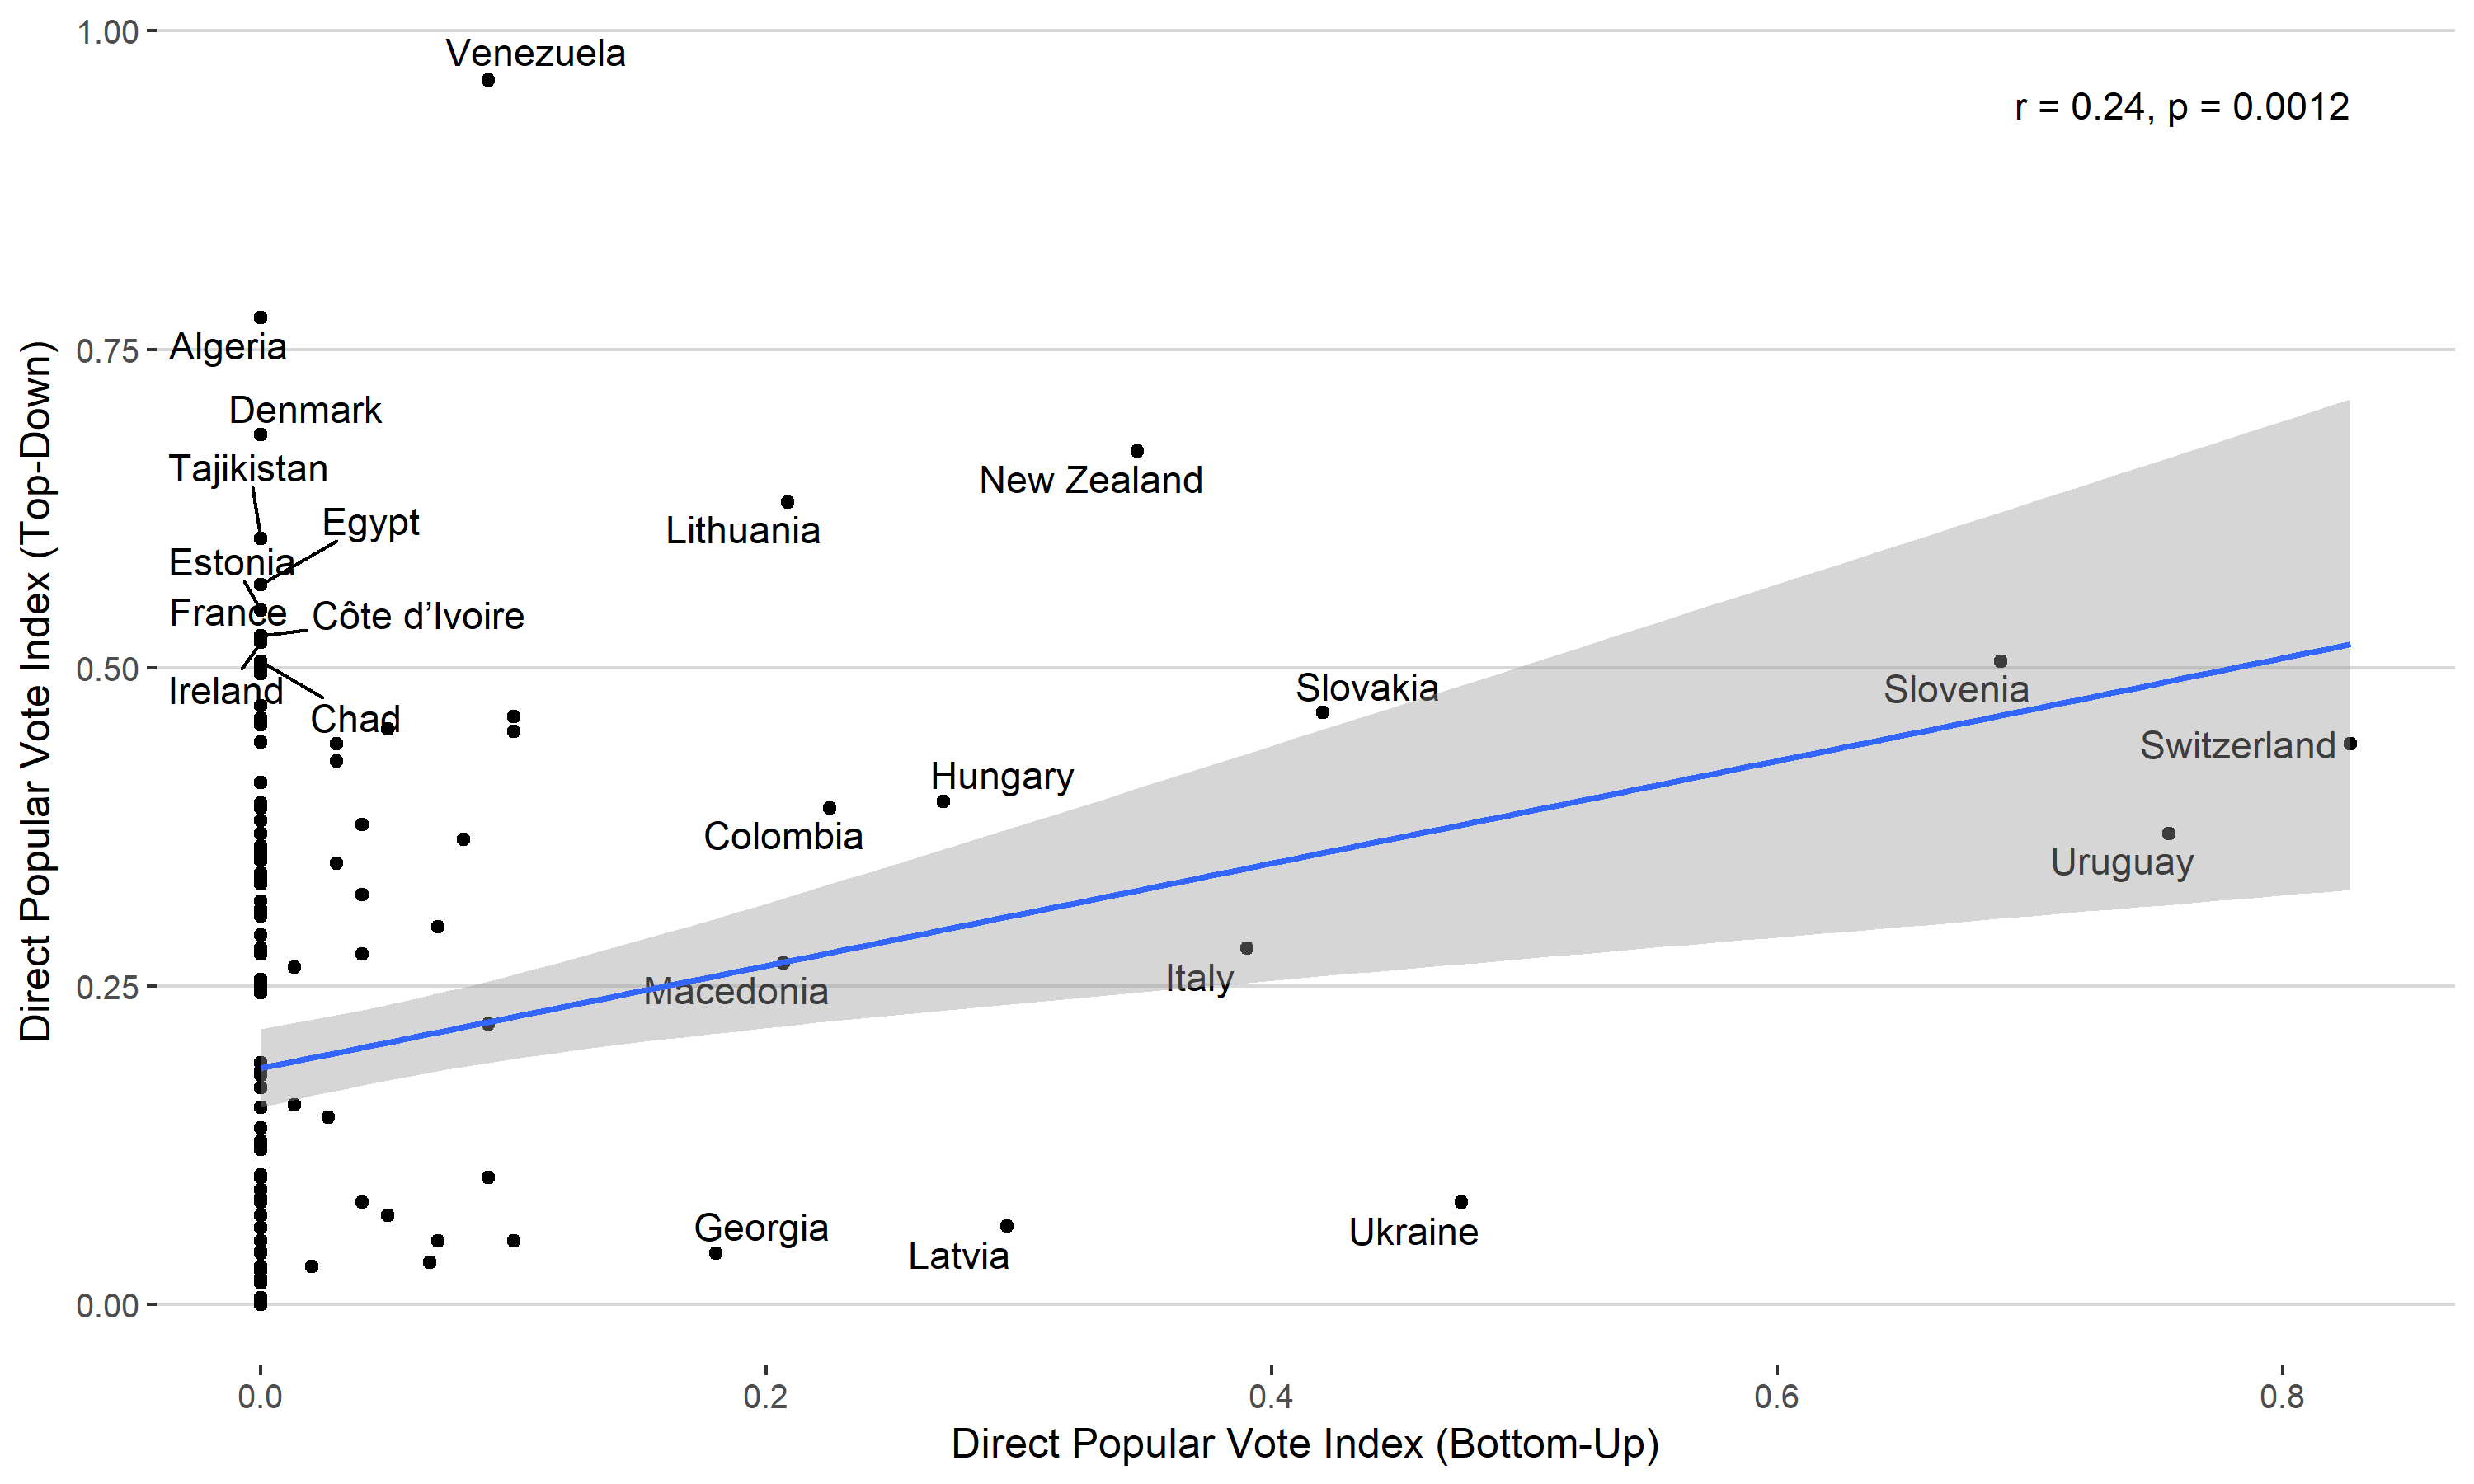
\includegraphics[width=\textwidth]{images/altman_tpbu.png}
    \flushright
    {\scriptsize Based on own calculations. \par}
\end{figure}


\end{document}
